\documentclass[12pt, a4paper]{article}
\usepackage{caption}
\captionsetup[figure]{name=Resim}
\captionsetup[table]{name=Tablo}
\usepackage{graphicx}
\usepackage{amsmath}
\renewcommand{\refname}{  Kaynakçalar}
\graphicspath{ {./images/} }
%opening
\usepackage{url}
\title{ Yapay Zeka Dersi Proje Tasarım Raporu}
\author{Celal ALTIN}
\date{\today}

\begin{document}
	\textbf{KÜTAHYA SAĞLIK BİLİMLERİ ÜNİVERSİTESİ}\centering\\
	\textbf{Bilgisayar Mühendisliği}\centering
	\begin{figure}[!h]
		\centering
		
\includegraphics{ksbu.png}
	\end{figure}
	\thispagestyle{empty}
	
	\maketitle\raggedright
	\maketitle\raggedright
	\maketitle
	Bu çalışma Yapay Zeka dersi final raporunu içermektedir. 
	
	
	\newpage
	\section{Giriş}
	2019 yılında başlayan COVID-19 salgını dünya çapında ciddi sağlık, ekonomik ve sosyal etkilere yol açmıştır.(Mart 2022 de yayınlanan bir habere göre \cite{haber1} dünyada ölüm sayısının 18 milyonu aştığı hesaplanıyor, bu sayı ülkemizde ise Sağlık bakanlığının verilerine göre 31.05.2022 tarihine kadar 98.965 kişinin hayatını kaybetti yönünde.)Bugün bile bu etkilerin sonuçları geçmiş değildir.\\
	\begin{figure}[!htbp]
		{
			\caption{Dunya Covit Haritasi \cite{site1}}
			\centering
			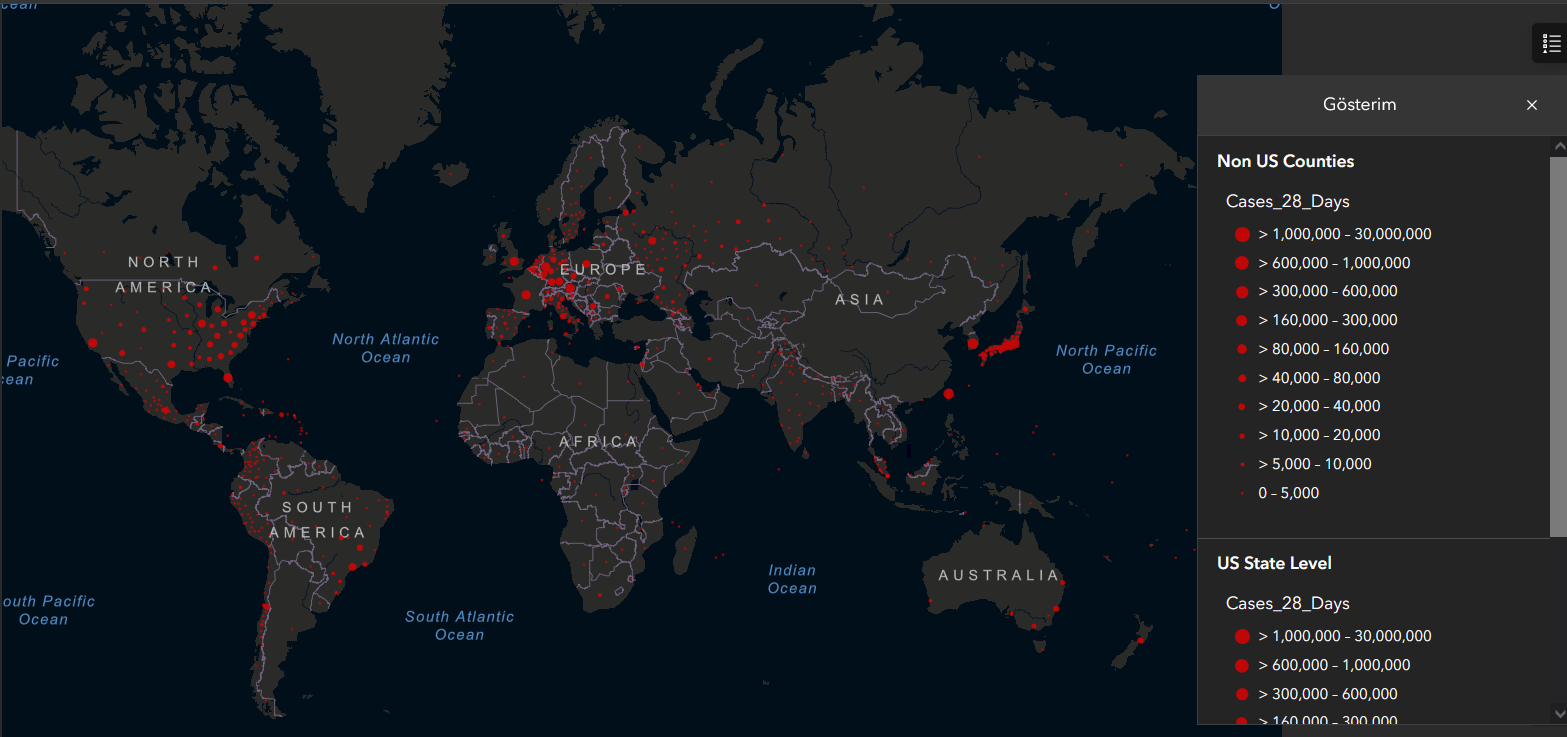
\includegraphics[angle=0, width=\textwidth]{hastalikdunya.png}
			\label{Dunya Covit Haritasi}
		}
		
		
	\end{figure}
	Dünya çapındaki bu problemi daha iyi anlayabilmek ve ileride olası hastalıklarda daha etkili mücadele edebilmek için bilgisayar(Makine öğrenmesi kulkanılarak yapılan bir araştırmaya göre sosyal medyanın da etkisiyle aşıya olan olumlu bakış artmıştır \cite{article} ) ve bilgisayar özelinde yapay zeka teknolojisinden faydalanmak en akılcı yöntemlerden birisidir.Bende bu projemde çeşitli kaynaklardan bulduğum Covit-19 verilerini kullanarak olası bir salgın hastalık dumunda gerçekleşebilecek seneryoyu gün yüzüne çıkartmayı amaçlıyorum.
	
	\section{Literatür Araştırması}
	Koronavirüs, 2019 yılının Aralık ayında ilk olarak Çin’in Wuhan kentinde ortaya çıkmış ve 11 Mart 2020’de Dünya Sağlık Örgütü tarafından pandemi olarak ilan edilmiştir. Vaka sayılarını kontrol altına almak için pek çok ülke karantina, sokağa çıkma yasağı ve sosyal alanların bir süreliğine kapatılması gibi çeşitli önlemler almıştır. Doğrulanmış vaka tahminlemesi pandemide olası planlamalar için büyük önem taşımaktadır. Gelecek verilerinin gerçeğe en yakın bir şekilde tahminlenmesi; pandemi döneminde lojistik, tedarik, hastane personel ve malzeme planlaması için kullanılabileceği gibi aşılama senaryolarında da girdi olarak kullanılabilir. Literatürde doğrulanmış vaka tahmininde makine öğrenmesi, bölmeli model, zaman serisi analizi gibi pek çok yöntem kullanarak tahminleme yapılan çalışmalar vardır. Bu çalışmada, Amerika Birleşik Devletleri’ndeki doğrulanmış vaka sayılarını kullanarak gelecek günlerdeki vaka tahminlerini çeşitli makine öğrenmesi modelleri yapılmıştır. Python ve R programlama dili kullanılarak yapılan tahminlemeler Prophet, Polinom Regresyon, ARIMA, Doğrusal Regresyon ve Random Forest modelleri ile yapılmıştır. Test verisiyle tahmin edilen verilerin performansları ortalama mutlak yüzde hatası (MAPE), ortalama karekök sapması (RMSE) ve ortalama mutlak hata (MAE) kullanılarak değerlendirilmiştir  \cite{article_855113}.\\ 
	PCA(Veri boyutunu azaltma yöntemleri sınıflandırma yapmak için
	harcanan zamanı ve bazı durumlarda sınıflandırma hatasını
	azaltmaya yardımcı olur. Zaman kritik
	uygulamalarda öznitelik elde etme evresinde harcanan zamanı
	azaltmak için, öznitelik seçme yöntemleri, tüm giriş
	değerlerinin ölçülmesini gerektiren boyut indirgeme
	yöntemlerine tercih edilir\cite{genc2007new}) yöntemi kullanıldığında doğruluk değeri en yüksek RF algoritmasında,
	duyarlılık ve kesinlik değeri en yüksek SMV algoritmasında saptanmıştır. Bu
	yöntemin kullanılması sonucunda en düşük doğruluk NB algoritmasında,
	duyarlılık ve kesinlik değerleri en düşük NB ve DT algoritmalarında elde
	edilmiştir\cite{article_1031070}.
	\begin{figure}[!htbp] 
		\caption{Dogruluk Tablosu}
		\centering
		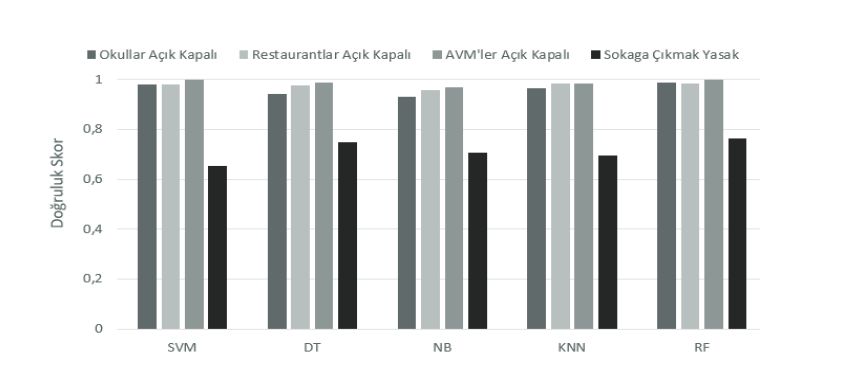
\includegraphics[angle=0, width=\textwidth]{dogruluk.png}
		\label{dogruluk}
	\end{figure}
	\newpage
	\section{Metodoloji}
	Projeni şematik planı aşağıdaki şekildedir.
	\begin{figure}[!htbp]
		\caption{GANTT CHART}
		\centering
		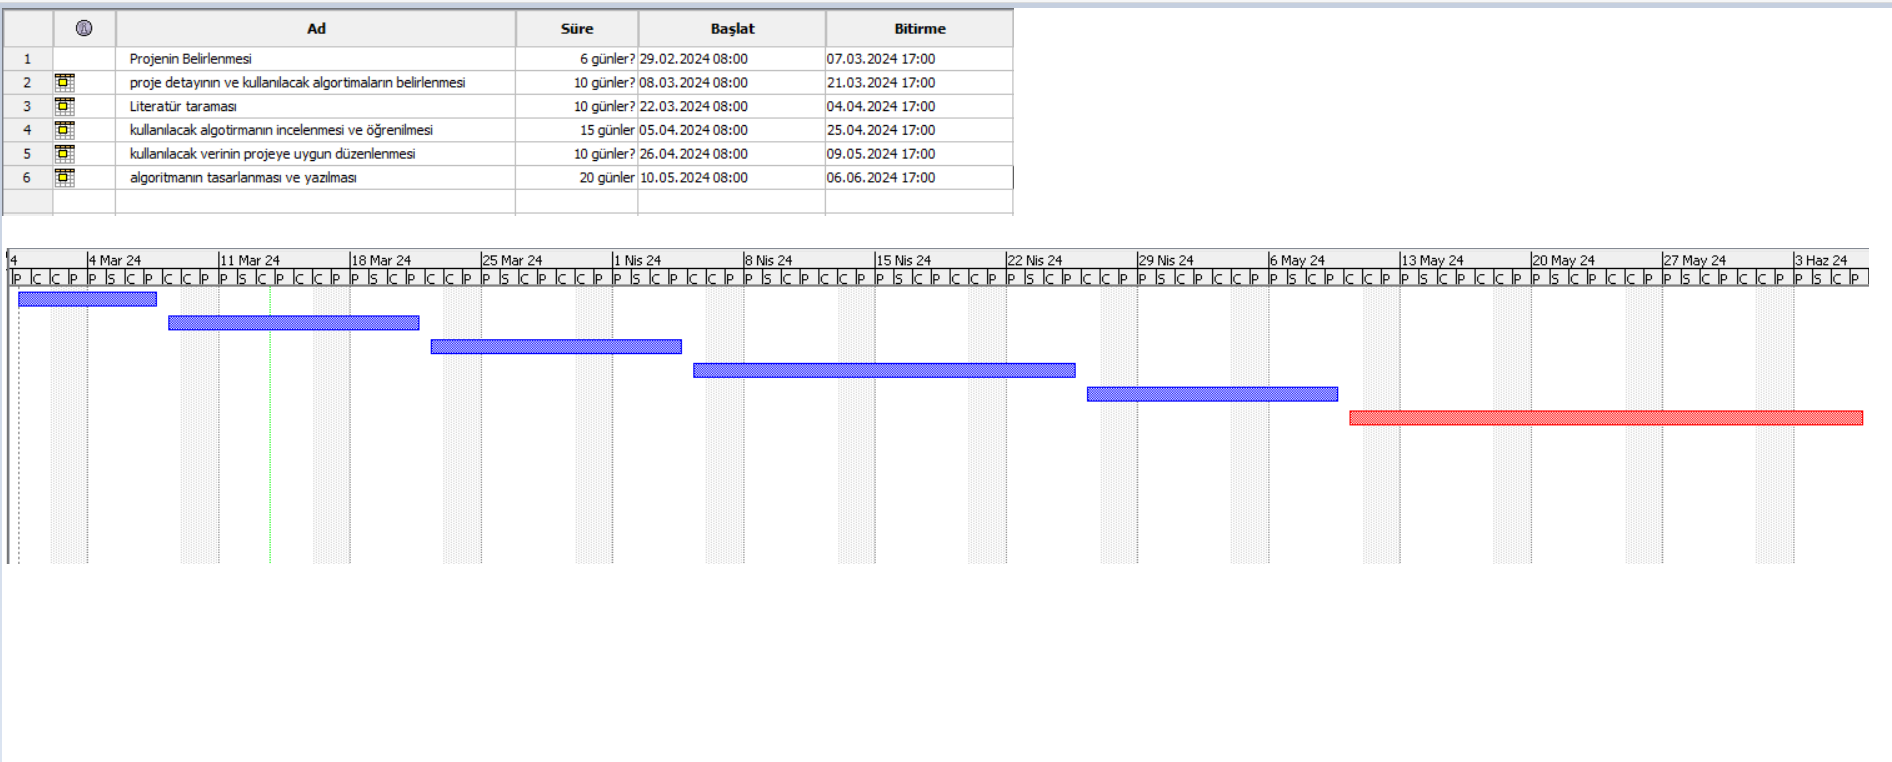
\includegraphics[ width=\textwidth]{gantt.png}
		\label{gantt}
	\end{figure}
	
	Projede kullanacağımız veriler gün veya haftalık olarak pozitif hasta sayısını, vefat edenlerin sayısını, kullandığımız verilerdeki insanların yaşadığı şehrin yada ülkenin nüfusunu, iyileşen sayısını,toplam test sayısı gibi parametreleri içermelidir.
	
	Veri işleme
	Normalizasyon işlemi- Araştırmalarda veri setlerinde verilerin
	bütünlüğünün sağlanması, veri tekrarının önlenmesi ve veri bütünlüğünün
	korunması ile performansının artırılması için normalizasyon yapılmaktadır.
	Daha sonra Çapraz doğrulama (Çapraz doğrulama, makine öğrenimi
	modellerinin başarı derecesini ortaya koymak için kullanılan yöntemdir.
	Çapraz doğrulama algoritma performansı hakkında bilgi verirken, verilerin
	daha verimli kullanılmasını sağlar.\cite{article_1031070})-yöntemi kullanılacaktır.
	Daha sonra PCA yöntemi kullanılarak veri kümesini azalttıktan sonra RF(Random Forest) algoritmasına beslenecektir.
	
	
	\section{Kullanılacak veri}
	
	Projemde iki farklı veri kaynağından faydalandım.Bunlardan ilki T.C. Sağlık Bakanlığından alınmış verilerdir.\cite{siteSaglik}.Verilerimiz 11.03.2020-31.05.2022 tarihleri arasında alınmış 813 farklı kayda sahiptir.Bu veriler Toplam Vaka, Günlük Vaka, Toplam Hasta, Gunluk Hasta, Toplam Vefat, Gunluk Vefat, Toplam iyilesen, Gunluk iyilesen, Gunluk Test şeklinde etiketlenmiştir.  \newline İkinci olarak ise Our World in Data kaynağından faydalanılmıştır\cite{owidcoronavirus}.
	\section{Yöntem}
	Olası bir salgın hastalık durumunda oluşabilecek sonuçları tahmin etmede fikir vermesi ve
	projemin \% 90 nın üzerinde doğrulukla sonuçlanması.
	\newpage
	Çalışmamızda Random Forest algoritmasını kullanılacağından bahsedilmişti.Random Forest algoritması Denetimli Öğrenme algoritmaları sınıfına ait bir algoritmadır.İnternete Random Forest algoritması yazıldığında karşınıza Random Forest regresyon(Regression) ve Random Forest sınıflandırma (Classification) algoritmaları çıkacaktır.
	\begin{figure}[!htbp] 
		\caption{ Machine Learning Algorithms }
		\centering
		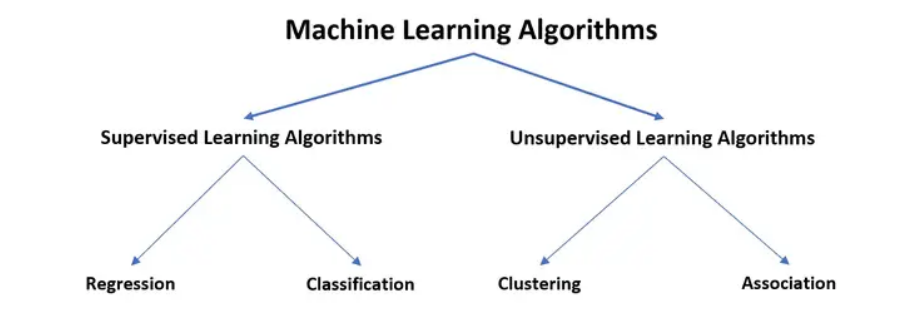
\includegraphics[angle=0, width=\textwidth]{resim3.png}
		
	\end{figure} 
	\newline Regresyon ve sınıflandırma farkından bahsetmeden önce denetimli öğrenme ve denetimsiz öğrenme algoritmaları arasındaki farktan bahsetmek daha sağlıklı olacaktır.\\
	\textbf{Denetimli Öğrenme Algoritması:} Denetimli Öğrenme algoritmasındaki en önemli nokta etiketli bir veri kümesi (labeled dataset) kullanılmasıdır. Yani hangi verinin hangi bilgiye karşılık geldiği bilindiğinden bilinen bir girdi seti ile bunlara denk gelen çıktıları alıp algoritmanın daha önce hiç görmediği (eğitimde kullanılmayan) yeni verilere en uygun çıktıları üretmek için kullanılan bir makine öğrenmesi modelidir.\cite{site2}
	\newpage
	\begin{figure}[!htbp] 
		\caption{ Denetimli Öğrenme  }
		\centering
		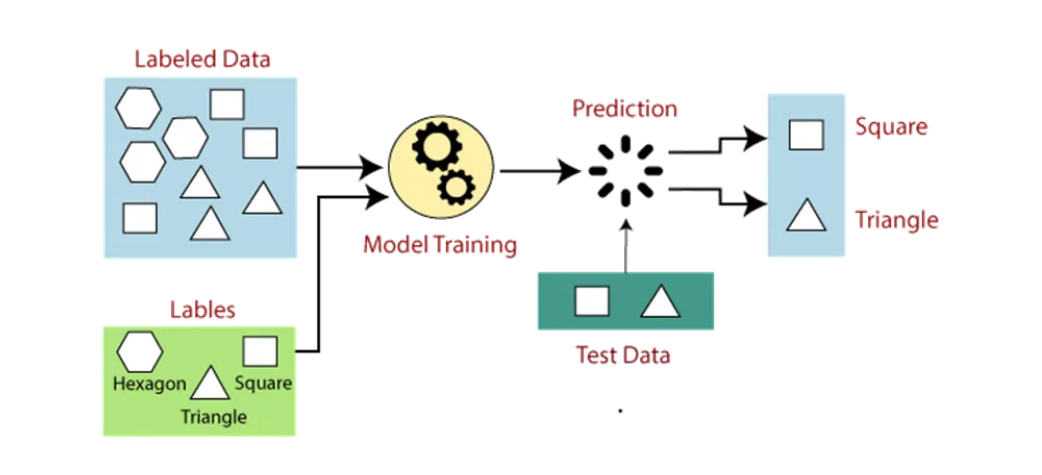
\includegraphics[angle=0, width=\textwidth]{resim1.png}
		
	\end{figure} 
	
	\textbf{Denetimsiz Öğrenme Algoritması:} Denetimsiz Öğrenmede ise etiketsiz veriler vardır. Bu etiketsiz veriler arasındaki gizli kalmış yapıyı/örüntüyü bulmaya çalışarak kendi kendine öğrenme biçimi sergilenir.\newline
	
	Denetimli öğrenme genellikle Regresyon ve Sınıflandırma problemlerine uygulanırken, denetimsiz öğrenme Kümeleme (Clustering) ve İlişkilendirme (Association) problemlerine uygulanır.
	\begin{figure}[!htbp] 
		\caption{ Denetimsiz Öğrenme  }
		\centering
		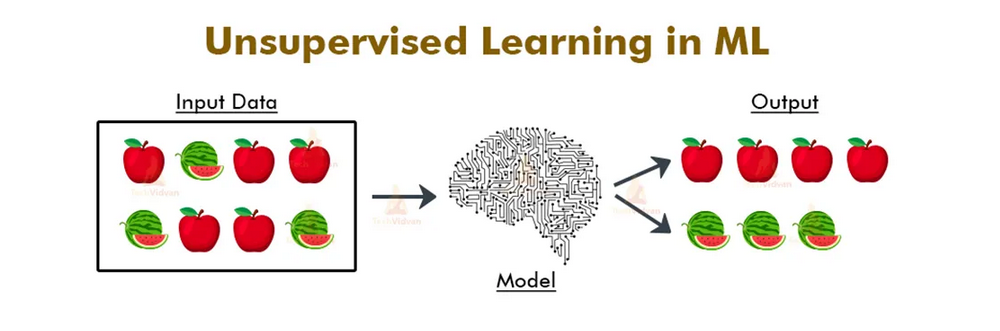
\includegraphics[angle=0, width=\textwidth]{resim2.png}
		
	\end{figure} 
	\newline
	Yukarı da da söylediğimiz gibi Random Fores algoritması araştırıldığında Random Forest regresyon ve Random Forest Sınıflandırma algoritmaları ile karşılaşılacak.Regresyon ve Sınıflandırma algoritmalarına biraz daha açıklık getirmemiz gereklidir.\newline
	\textbf{Regresyon(Regression) Nedir ?}
	
	
	Regresyon bağımlı bir değişken ile bağımsız bir değişken arasındaki ilişkinin, ortadan kaldırılması için kullanılan istatistiksel bir yöntemdir. Evet, regresyonun bu teorik açıklaması size karmaşık gelmiş olabilir. Gelin biz bunu daha basit haliyle açıklayalım. Buradaki değişkenler(x ve y arasında, x → deneyim yılı, y → maaş olarak düşünebilirsiniz) arasında sebep-sonuç ilişkisi bulmaya çalışırız ve bulduğumuz bu ilişkiye göre tahminler yaparız.
	
	En basit haliyle regresyonu açıklayacak olursak, bir veri setinde sayısal tahmin yapıyorsak “regression” algoritmalarını kullanırız.
	
	Örnek → Maaş tahmini, yaşa göre boy tahmini, çalışma süresine göre alınan not tahmini gibi örnekler verebiliriz. \newline
	
	\textbf{Sınıflandırma(Classification) Nedir ?}
	
	
	Regression problemlerinde tahmin edeceğimiz y kolonunda sayısal değerler vardı. Biz x değerlerini yani giriş değerini kullanarak sayısal tahminler yapmaya çalışıyorduk. Sınıflandırma problemlerinde ise x(giriş değerleri) değerlerini kullanarak kategorik olarak y sınıfını tahmin etmeye çalışırız.\cite{site3}
	
	
	
	\begin{figure}[!htbp] 
		\caption{ Regresyon ve Sınıflandırma  }
		\centering
		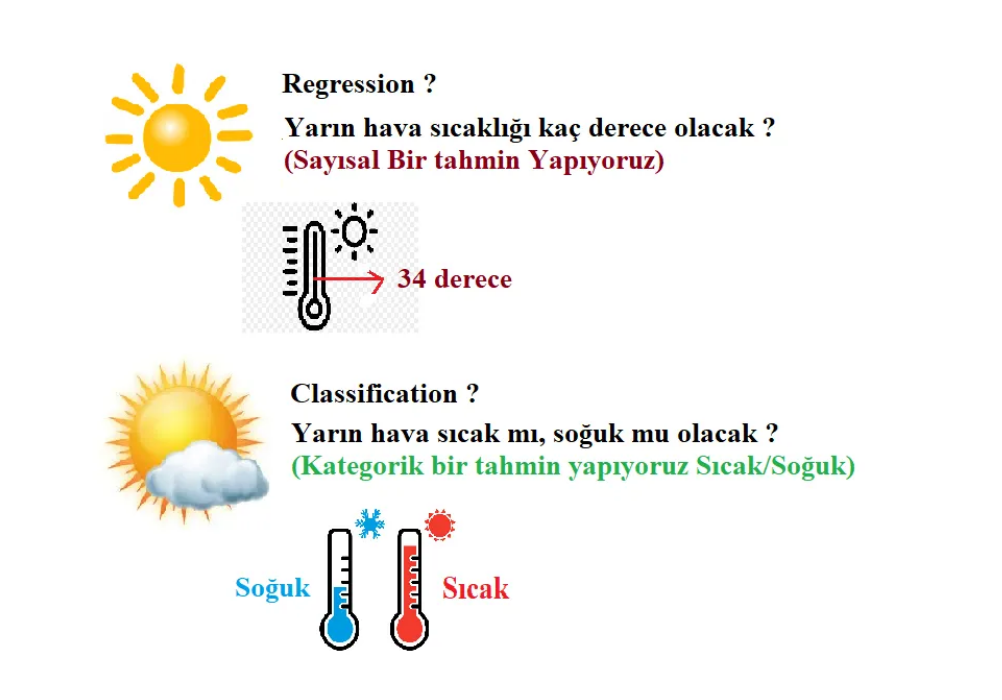
\includegraphics[angle=0, width=\textwidth]{resim4.png}
		\label{dogruluk}
	\end{figure} 
	
	
	\newpage \textbf{Random Forest (Rassal Orman) Algoritması:} 
	Sınıflandırma işlemi esnasında birden fazla karar ağacı üreterek sınıflandırma değerini yükseltmeyi hedefleyen bir algoritmadır. Bireysel olarak oluşturulan karar ağaçları bir araya gelerek karar ormanı oluşturur. Buradaki karar ağaçları bağlı olduğu veri setinden rastgele seçilmiş birer alt kümedir.
	\begin{figure}[!htbp] 
		\caption{ Single Decision tree and Random Forest }
		\centering
		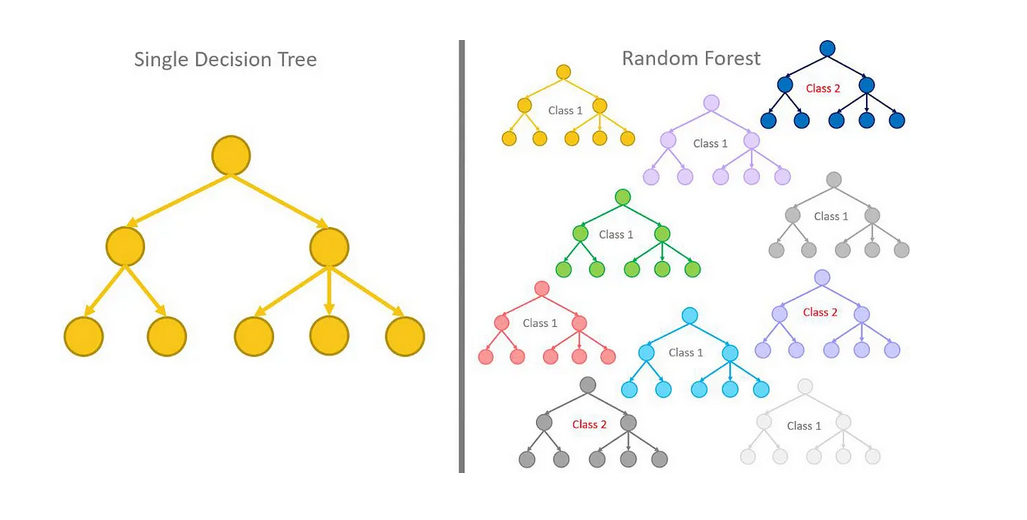
\includegraphics[angle=0, width=\textwidth]{resim5.png}
		
	\end{figure} \newline
	Fark ettiyseniz Random Forest karar ağaçlarının bir nevi birleşiminden oluşan bir algoritma.\cite{site4}
	\newpage
	
	
	\begin{figure}[!htbp] 
		\caption{ Random Forest }
		\centering
		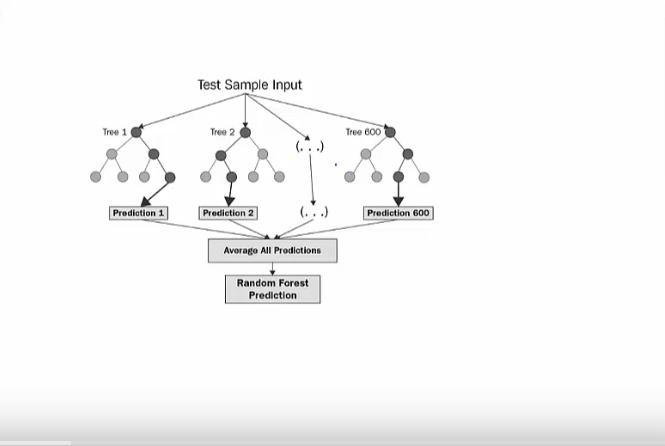
\includegraphics[angle=0, width=\textwidth]{resim6.png}
		
	\end{figure} 
	
	
	
	
	\maketitle
	
	Random Forest algoritmamı uygulayacağım veriler aşağıda gösterilmiştir.
	\begin{figure}[!htbp] 
		\caption{Covit Verileri}
		\centering
		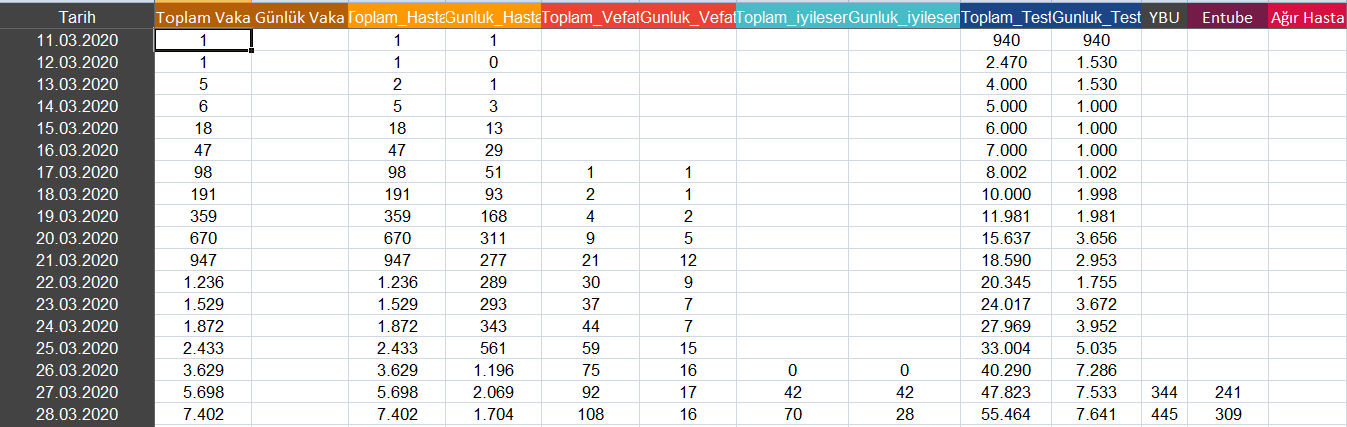
\includegraphics[angle=0, width=\textwidth]{4.0.png}
		
	\end{figure} 
	\newline
	Verilerim gün bazında Türkiye için Toplam Vaka, Günlük Vaka, Toplam Hasta, Günlük Hasta, Toplam Vefat, Günlük Vefat, Toplam İyileşen, Günlük İyileşen, Toplam Test, Günlük Test, Yoğun Bakım Ünitesi ve Ağır Hasta parametrelerinden 812 kayıt içermektedir.
	
	\begin{figure}[!htbp] 
		\caption{Kodlar}
		\centering
		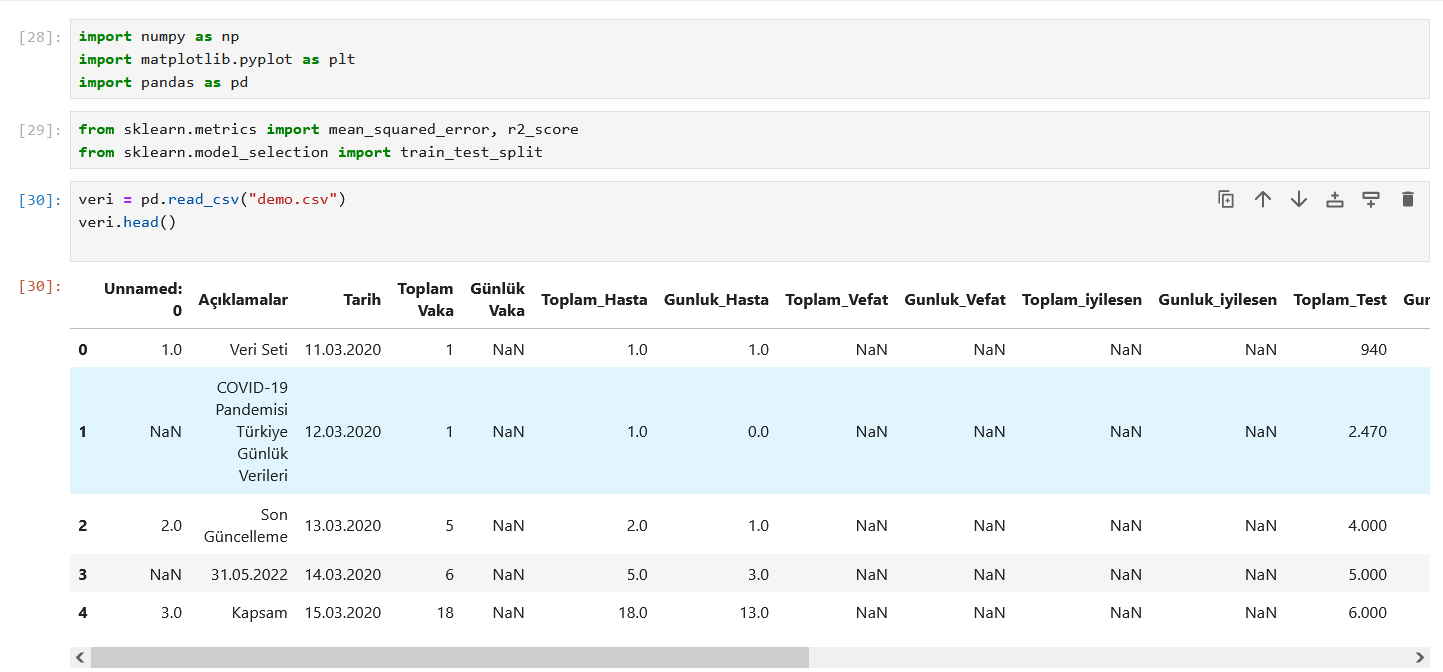
\includegraphics[angle=0, width=\textwidth]{5.0.png}
		
	\end{figure} 
	
	Öncelikler kullacağımız kütüpheneleri çalışmamıza ekliyoruz ve pandas kütüphanesinin read.csv fonksiyonuyla verilerimizi içeri alıyoruz.\newline
	Daha sonra verilerimizi incelemek ilk 5 veriyi getiriyoruz.
	
	\begin{figure}[!htbp] 
		\caption{Kodlar2}
		\centering
		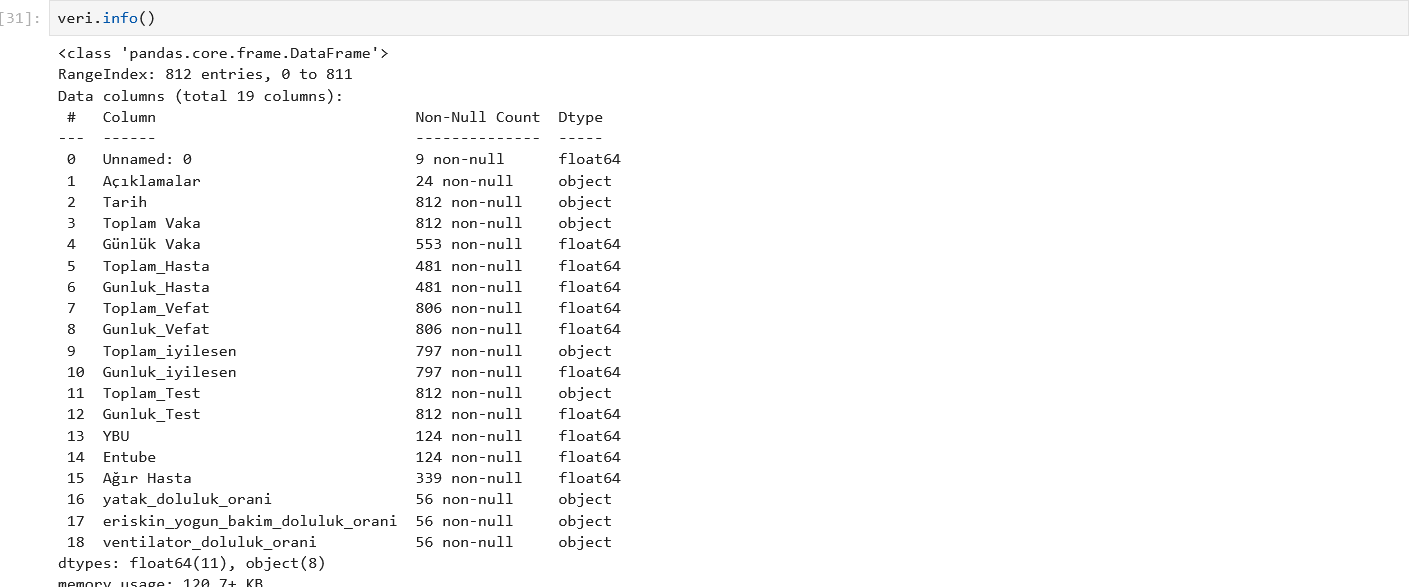
\includegraphics[angle=0, width=\textwidth]{6.0.png} 
		
	\end{figure} 
	\newpage
	Verilerimizi detaylı incelemek için veri.info() metotunu kullanıyoruz.
	
	\begin{figure}[!htbp] 
		\caption{Kodlar3}
		\centering
		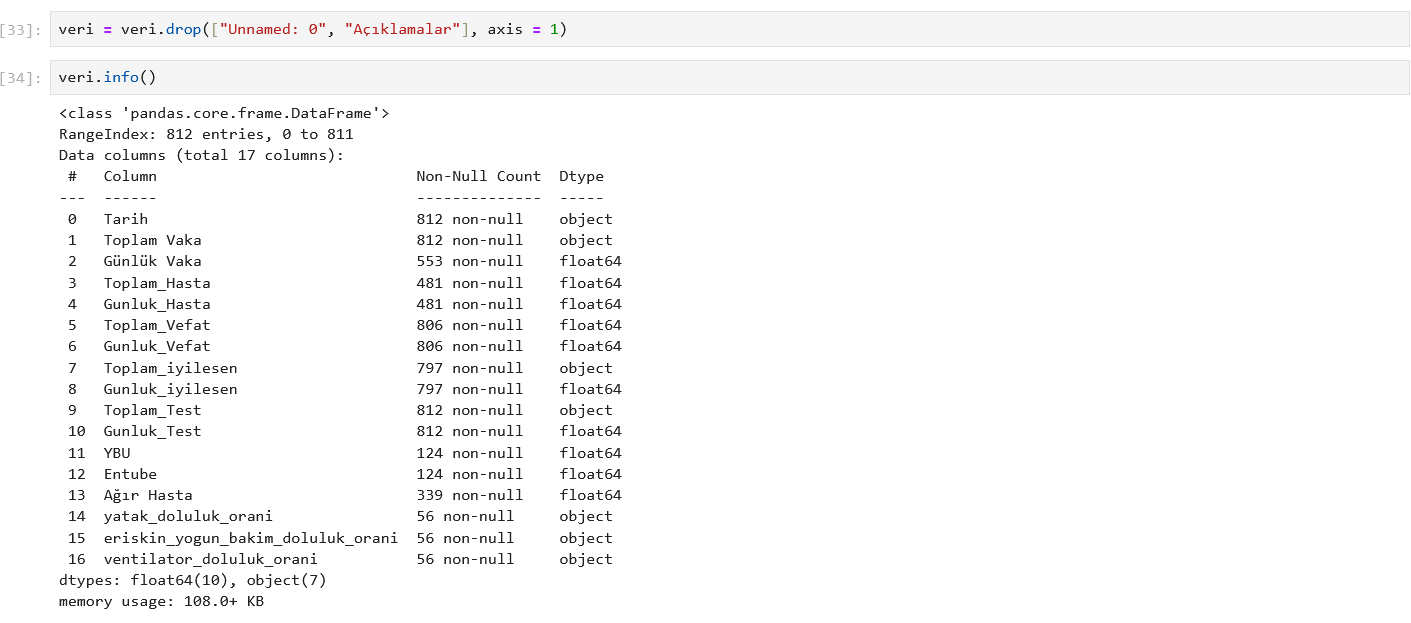
\includegraphics[angle=0, width=\textwidth]{7.0.png} 
		
	\end{figure}
	Daha sonra kullanılmayacak olan Unnamed : 0 ve Açıklamalar sütununu sililyoruz ve tekrar kontrol ediyoruz.
	
	\begin{figure}[!htbp] 
		\caption{Kodlar4}
		\centering
		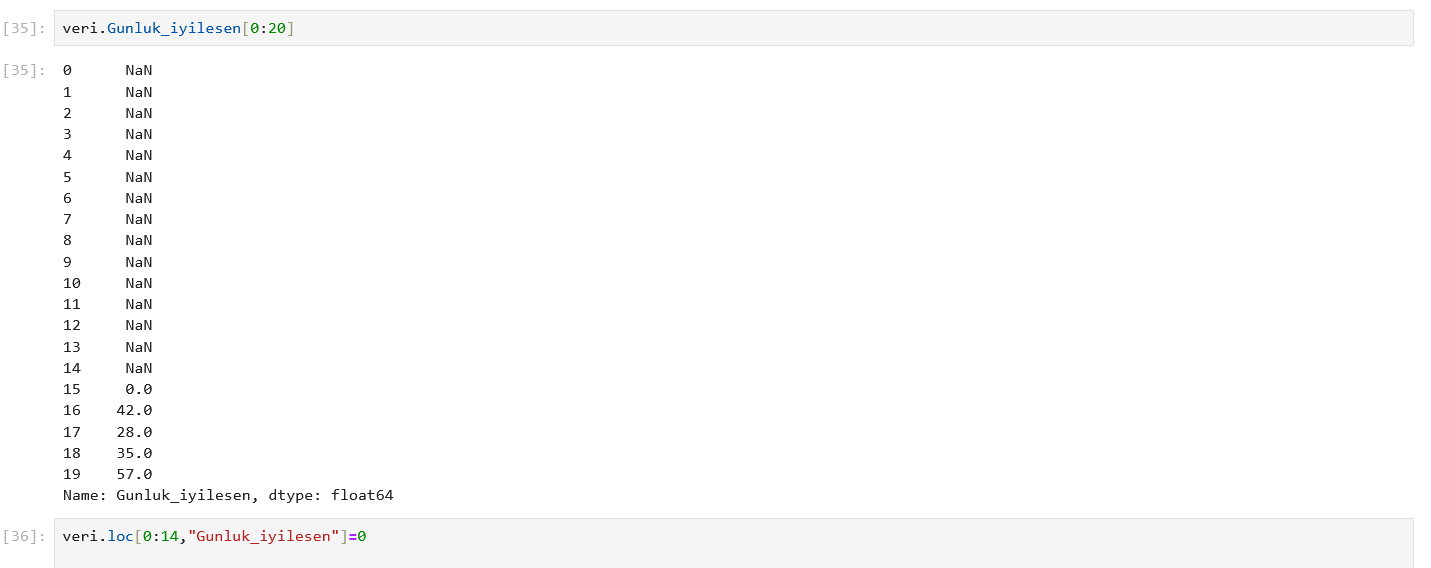
\includegraphics[angle=0, width=\textwidth]{8.0.png} 
		
	\end{figure}
	
	\newpage
	Günlük iyileşen sütununa baktığımızda ilk 15 verimizin NaN değere sahip olduğunu görüyoruz.Algoritmamızda kullanacağımız için 2 değerini atıyoruz.
	\begin{figure}[!htbp] 
		\caption{Kodlar5}
		\centering
		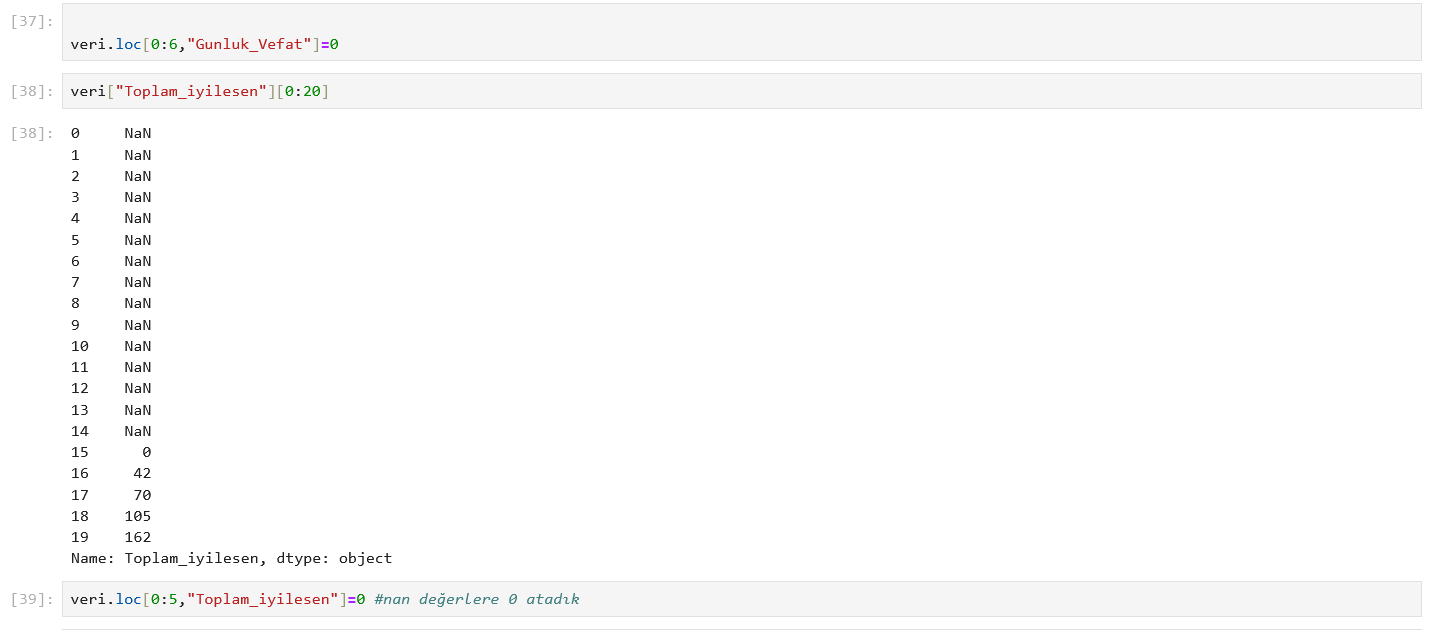
\includegraphics[angle=0, width=\textwidth]{9.0.png} 
		
	\end{figure}
	Daha sonra aynı işlemi Günlük vefat ve Toplam iyileşen sütunlarımıza da yapıyoruz.
	
	\begin{figure}[!htbp] 
		\caption{Kodlar6}
		\centering
		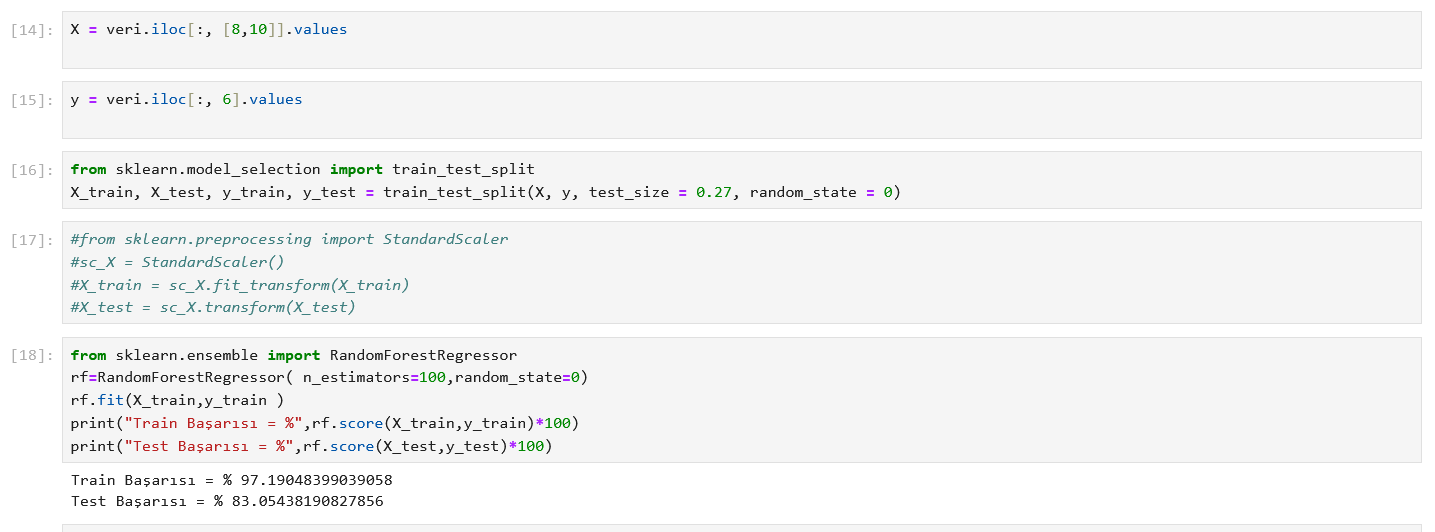
\includegraphics[angle=0, width=\textwidth]{10.0.png} 
		
	\end{figure}
	\newpage
	Daha sonra eğitimde ve testte kullanılacak verilerimizi ayırıyoruz. Verilerimizin \%27 sini test için ayırıyoruz.100 adet karar ağacı kullanıyoruz.Eğitim başarımını \%97 test başarımını \%83 olarak buluyoruz.
	
	\begin{figure}[!htbp] 
		\caption{Kodlar7}
		\centering
		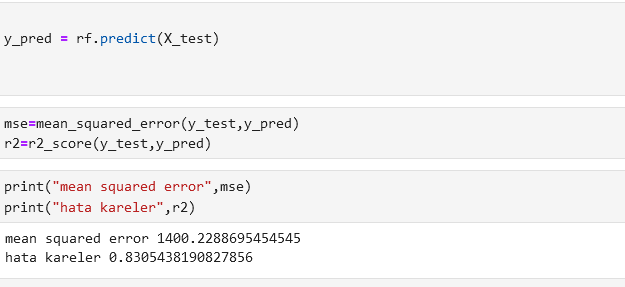
\includegraphics[angle=0, width=\textwidth]{11.0.png} 
		
	\end{figure}
	\textbf{R Kare:} R kare, modeldeki bağımsız değişkenlere göre bağımlı değişkenin varyasyon oranını yani bağımlı değişkendeki değişkenliğin ne kadarının model tarafından açıklanabileceğini ölçer. Korelasyon katsayısının karesidir. R Kare aşırı uyum (overfitting) sorununu dikkate almaz. Regresyon modelinin çok fazla bağımsız değişkeni varsa model eğitim verilerine çok iyi uyabilir ama testte istenen başarıyı gösteremeyebilir. Bu nedenle Düzeltilmiş R Kare kullanılır. Düzeltilmiş R Kare modele eklenen ek bağımsız değişkenleri cezalandırır ve aşırı uyum sorununu çözer.\newline
	\begin{math} 
		\centering	\newline 1-\frac{Ssres}{SStot} 
	\end{math}\newline
	SSres: hata kareler toplamı\newline
	SStot: toplam kareler toplamı\newline
	\textbf{Ortalama Kare Hatası (Mean Squared Error (MSE)):} Ortalama Kare Hatası tahmin edilen sonuçlarınızın gerçek sayıdan ne kadar farklı olduğuna dair size mutlak bir sayı verir. Tek bir sonuçtan çok fazla içgörü yorumlayamazsınız, ancak size diğer model sonuçlarıyla karşılaştırmak için gerçek bir sayı verir ve en iyi regresyon modelini seçmenize yardımcı olur. \cite{site11}
	\begin{math} 
		\centering	\newline \frac{1}{n} * \sum_{}^{}(y-ypred)^2
	\end{math}	
	\newline n:Veri noktalarının sayısı.
	\newline y:Gerçek değerler.
	\newline ypred: Tahmin edilen değerler.
	\newline Daha Sonraki projemizi diğer veri setinden çektiğimiz veriler ile yapacağız.\cite{owidcoronavirus}
	\begin{figure}[!htbp] 
		
		\centering
		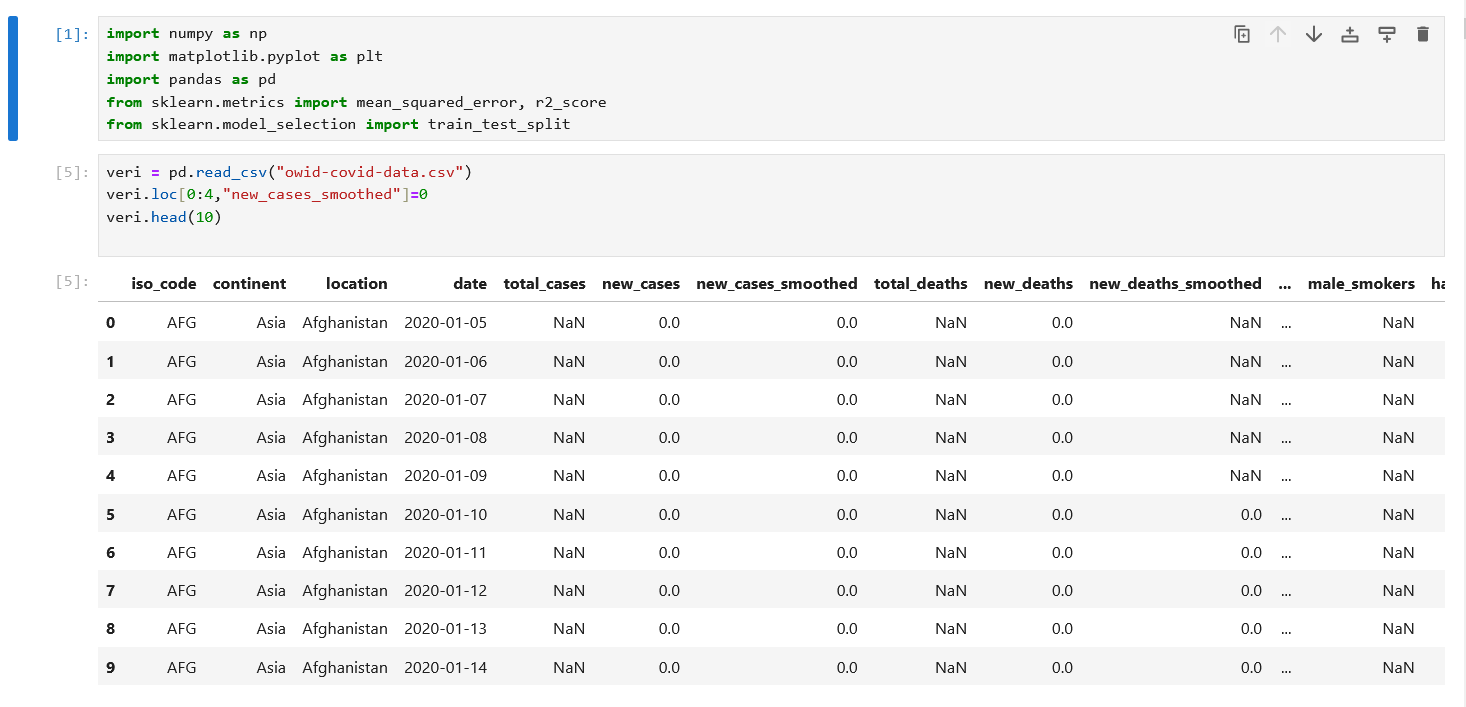
\includegraphics[angle=0, width=\textwidth]{1.png}
		\caption{Verilemizin Genel İncelenmesi}
		
		
	\end{figure} 
	\newline   Yukarıda gördüğünüz kodlarda kullanıcağımız kütüphaneleri projemize ekledik ve kullanacağımız verilerden new cases smoothed sütunundaki ilk 4 veri NaN değere sahip olduğu için 0 atadık ve daha sonra ilk 10 verimizi kontrol ettik.
	\begin{figure}[!htbp] 
		
		\centering
		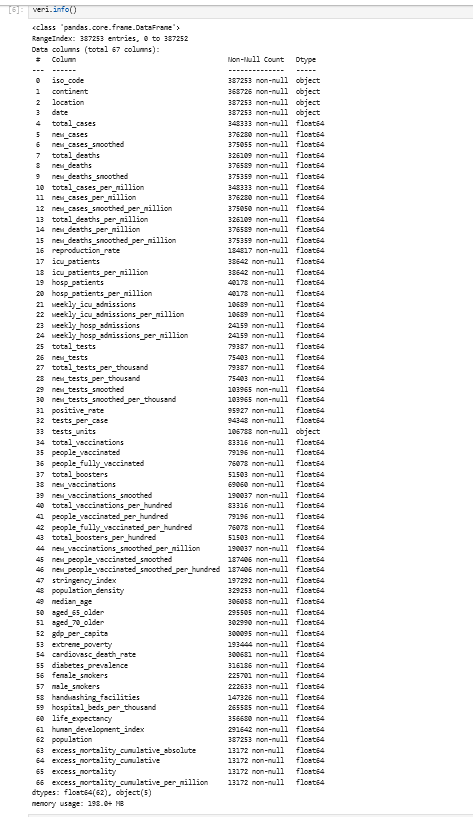
\includegraphics[angle=0, width=\textwidth]{2.png}
		\caption{Verilerimize Detaylı İncelenmesi}
	\end{figure}
	\newpage Hangi türden ne kadar veri olduğunu ve hangi sütun adı altında olduklarını inceledik. 
	\begin{figure}[!htbp] 
		
		\centering
		
\includegraphics[angle=0, width=\textwidth]{3.png}
		\caption{Afganistan için new cases sütununun seçilmesi}
	\end{figure}
	\newline İlk verilerimiz Afganistan'a ait verilerdir.Verilerimizi bir dataframe a atıp location kolonunda Afghanistan olan verilerimizi alıyoruz(Birden fazla ülkenin verileri aynı veri tabanında olduğu için).Daha sonra bağımlı değişkenlerimizde kullanmak  üzere new cases verilemizi ayıklayıp indeks numarası 7 nin katları olacak şekilde tekrar alıyoruz.Bunun sebebi ise verilerimizin her 7 günde güncellenmesi aradaki günlerde veri girilmemesi.
	\begin{figure}[!htbp] 
		
		\centering
		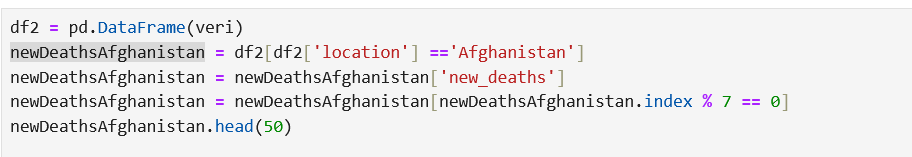
\includegraphics[angle=0, width=\textwidth]{4.png}
		\caption{Afganistan için new deaths sütununun seçilmesi}
	\end{figure}
	\newline Aynı işlemleri new deaths, new cases smoothed, diabetes prevalence, cardiovasc death rate ve population sütunlarımız içinde yapıyoruz.
	\begin{figure}[!htbp] 
		
		\centering
		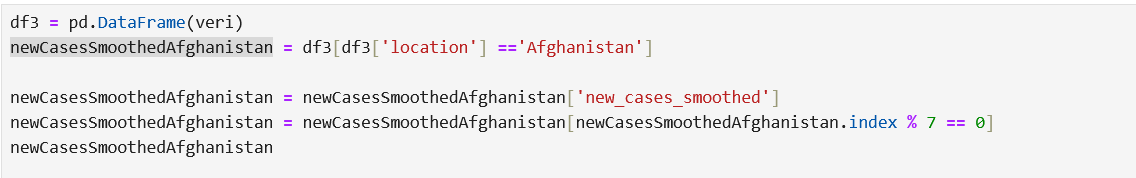
\includegraphics[angle=0, width=\textwidth]{5.png}
		\caption{Afganistan için new cases smoothes sütununun seçilmesi}
	\end{figure}
	\begin{figure}[!htbp] 
		
		\centering
		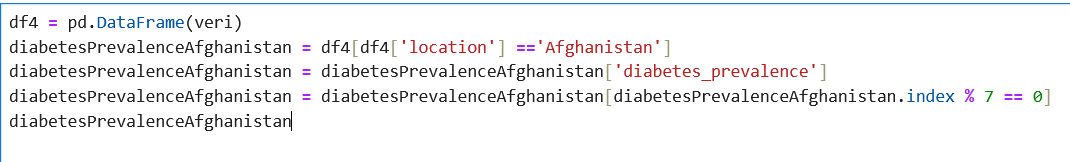
\includegraphics[angle=0, width=\textwidth]{6.png}
		\caption{Afganistan için diabetes prevalance sütununun seçilmesi}
	\end{figure}
	\begin{figure}[!htbp] 
		
		\centering
		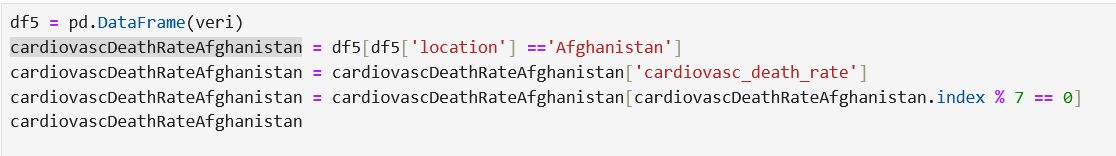
\includegraphics[angle=0, width=\textwidth]{7.png}
		\caption{Afganistan için cardiovasc death rate sütununun seçilmesi}
	\end{figure}
	\begin{figure}[!htbp] 
		
		\centering
		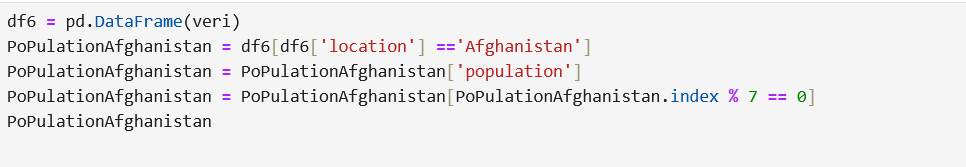
\includegraphics[angle=0, width=\textwidth]{8.png}
		\caption{Afganistan için population sütununun seçilmesi}
	\end{figure}
	\begin{figure}[!htbp] 
		
		\centering
		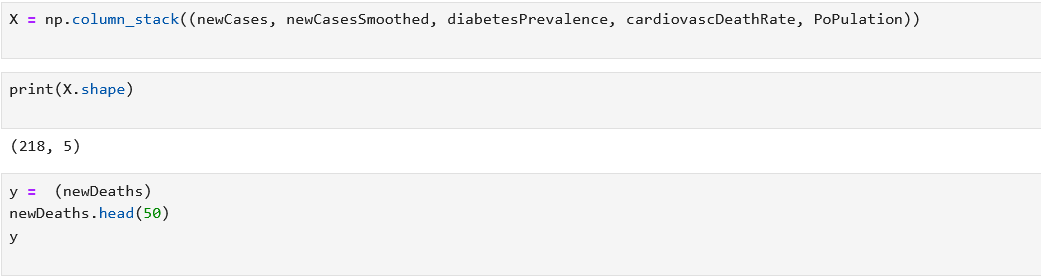
\includegraphics[angle=0, width=\textwidth]{9.png}
		\caption{Bağımlı ve bağımsız değişkenlerin oluşturulması}
	\end{figure}
	\newline
	\newpage
	Daha sonra projemizde kullanmak üzere bağımlı X ve bağımsız y değikenlerini oluşturuyoruz.Kodda da görüldüğü gibi bağımlı değişkenimiz new cases, new cases smoothed, diabetes prevalence, cardiovasc death rate ve population verilerimiz içerirken tahim edeceğimiz yani bağımsız değişkeinimiz new deaths verilerini içeriyor.En son olarak bağımlı ve bağımsız değişkenlerin boyutlarını kontrol etmemin sebebi satır sayılarının aynı olması gerektiğindendir.
	\newline
	\begin{figure}[!htbp] 
		
		\centering
		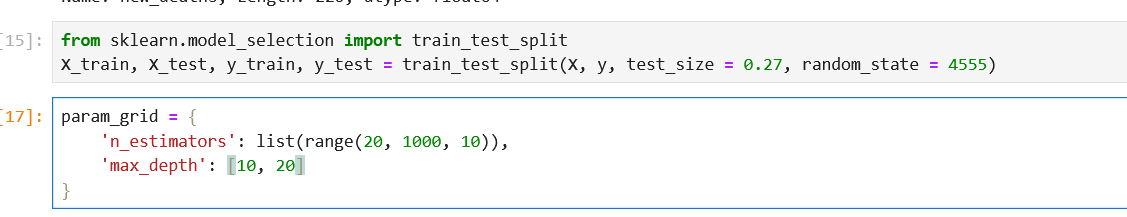
\includegraphics[angle=0, width=\textwidth]{10.png}
		\label{fig:yenietiket}
		\caption{Test, eğitim verilerinin ayrılması ve parametre ayarı.}
	\end{figure}
	\newline Yukarıdaki kodda test ve eğitim verilerimizi \%27 test verisi olacak şekilde ayırdık.Daha sonra en başarılı parametre ayarını bulmak için değişkenlerimizi tanımladık.
	
	\begin{figure}[!htbp] 
		
		\centering
		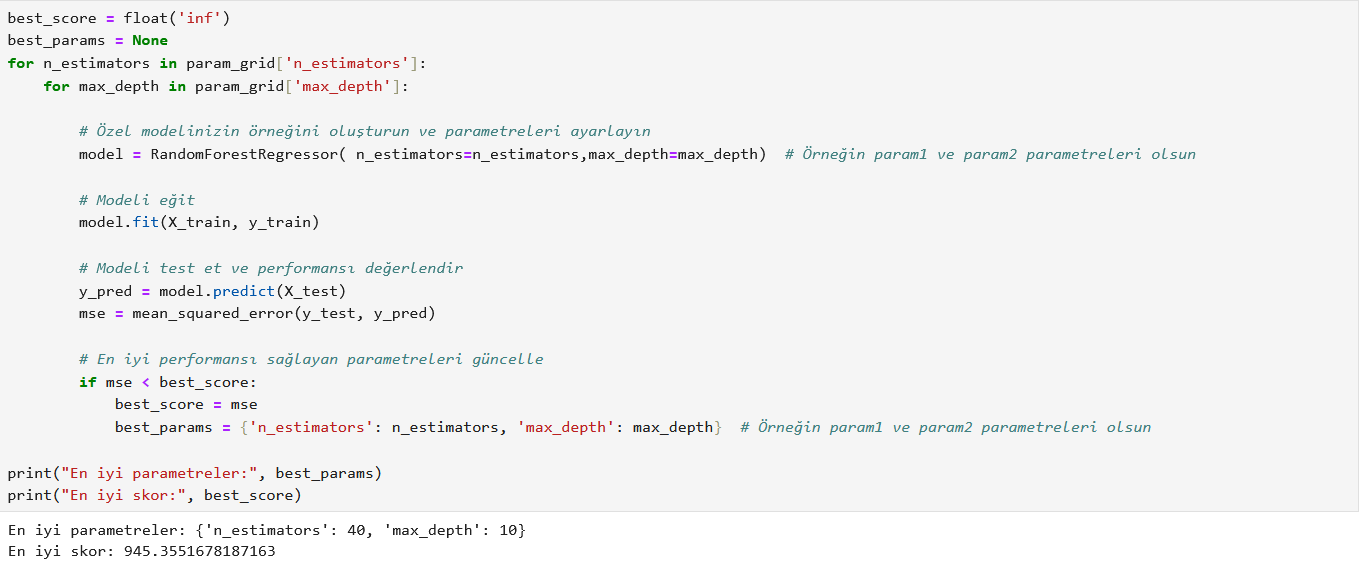
\includegraphics[angle=0, width=\textwidth]{11.png}
		\label{fig:yenietiket2}
		\caption{Test, eğitim verilerinin ayrılması ve parametre ayarı.}
	\end{figure}
	Yukarıdaki kodda Resim \ref{fig:yenietiket} da tanımladığımız değişkenleri kullanarak her değişkenin tüm kombinasyonlarını deneyerek mse sini hesaplıyoruz ve en skoru veren parametre değerlerini buluyoruz.
	
	
	\begin{figure}[!htbp] 
		
		\centering
		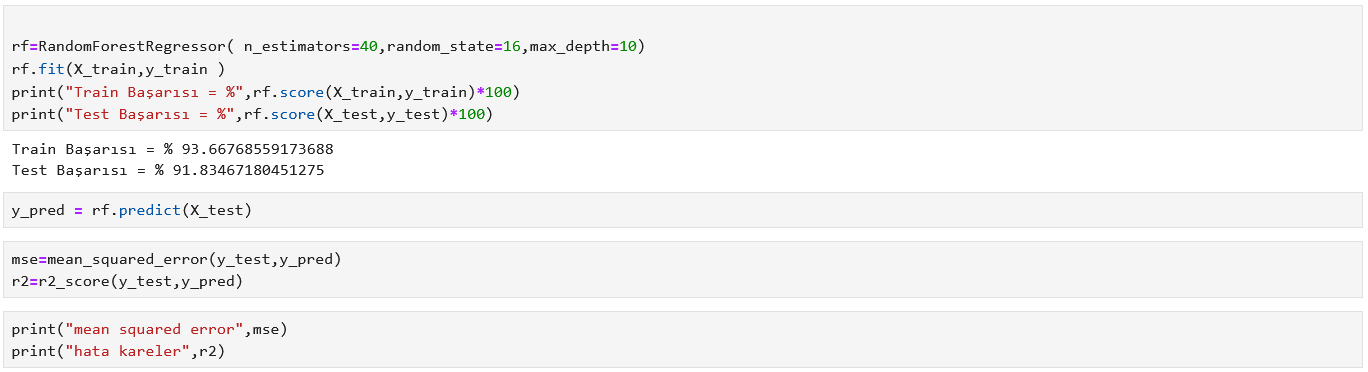
\includegraphics[angle=0, width=\textwidth]{13.png}
		\caption{Modelin eğitilmesi.}
	\end{figure}
	\newpage
	En son olarak Resim \ref{fig:yenietiket2} de elde ettiğimiz verilere göre modelimizi eğitiyoruz, mse ve r2 değerlerini hesaplıyoruz.
	\newline
	\newline
	Aynı işlemi veri tabanımızdaki Avustralya, Brezilya, ve Çin içinde yaptık.Lakin eğitim başarımları ve test başarımları tatmin edici seviyede değildi.
	
	\begin{figure}[!htbp] 
		
		\centering
		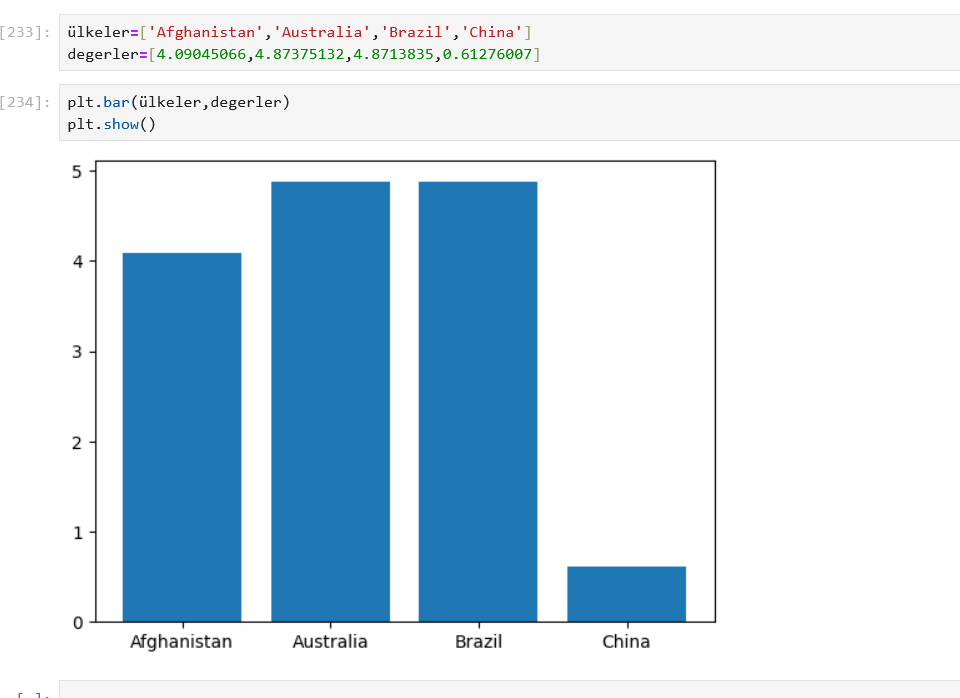
\includegraphics[angle=0, width=\textwidth]{14.png}
		\caption{4 Ülkenin Karşılaştırılması.}
	\end{figure}
	Yukarıdaki kodlarda 4 ülke için eğitilmiş modele beslediğimiz değerlerden (new cases = 100 ,new cases smoothed = 20, diabetes prevalence = 5, cardiovasc death rate=150, population = 1000000) elde ettiğimiz çıktılar karşılaştırılmıştır.
	\newline
	\begin{centering}
		
		\begin{tabular}{lll}
			\hline
			Ülkeler  & Eğitim başarımı & Test başarımı \\ \hline
			Afghanistan & \% 93.66 & \% 91.83 \\
			Australya1 & \% 87.35 & \% 35.51 \\
			Brezil & \% 93.18 & \% 54.74 \\
			China & \% 78.92 & \% 57.72 \\
			\hline
		\end{tabular}
	\end{centering}
	\newline Yukarıdaki tabloda projemde kullandığım ülke verilerin eğitim ve test başarımları verilmiştir.
	Geçen haftalarda Random Forest algoritmasıyla yaptığım çalışmayı Yapay Sinir Ağları(Neural Network) ile yapmaya çalışıyıyorum. Öncelikle yapay sinir ağlarını tanımakla başlamanın doğru olacağını düşünüyorum.
	\newline
	Yapay sinir ağları (YSA), insan beyninin bilgi işleme tekniğinden esinlenerek geliştirilmiş bir bilgi işlem teknolojisidir. YSA ile basit biyolojik sinir sisteminin çalışma şekli taklit edilir. Yani biyolojik nöron hücrelerinin ve bu hücrelerin birbirleri ile arasında kurduğu sinaptik bağın dijital olarak modellenmesidir. Nöronlar çeşitli şekillerde birbirlerine bağlanarak ağlar oluştururlar. Bu ağlar öğrenme, hafızaya alma ve veriler arasındaki ilişkiyi ortaya çıkarma kapasitesine sahiptirler. Diğer bir ifadeyle, YSA'lar, normalde bir insanın düşünme ve gözlemlemeye yönelik doğal yeteneklerini gerektiren problemlere çözüm üretmektedir. Bir insanın, düşünme ve gözlemleme yeteneklerini gerektiren problemlere yönelik çözümler üretebilmesinin temel sebebi ise insan beyninin ve dolayısıyla insanın sahip olduğu yaşayarak veya deneyerek öğrenme yeteneğidir. \cite{wikipedia}
	
	\begin{figure}[!h]
		\centering
		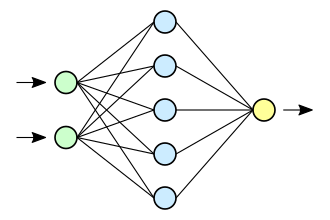
\includegraphics{4.7.png}
		\caption{Yapay Sinir Ağları örnek şeması.}
	\end{figure}
	Yapay sinir ağlarına diğer nöronlardan gelen ağırlıkları ile işlenmiş sinyaller giriş fonksiyonuna sokulur ve orada belirlenmiş işlemler yapılır(Toplama, çarpma, min-max bulma vb.).Daha sonra aktifleştime fonksiyonuna girer.Burada belli fonksiyonlardan geçerek eşik değerinden geçerse 1, geçmezse 0 tetiklenir.Output dan diğer nöronlara gönderilir.
	\begin{figure}[!h]
		\centering
		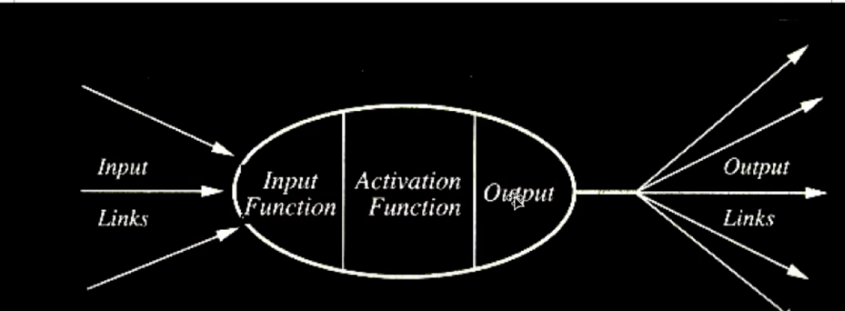
\includegraphics{4.2.png}
		\caption{Nöron yapısı.}
		\cite{youtube}
	\end{figure}
	
	\begin{figure}[!h]
		\centering
		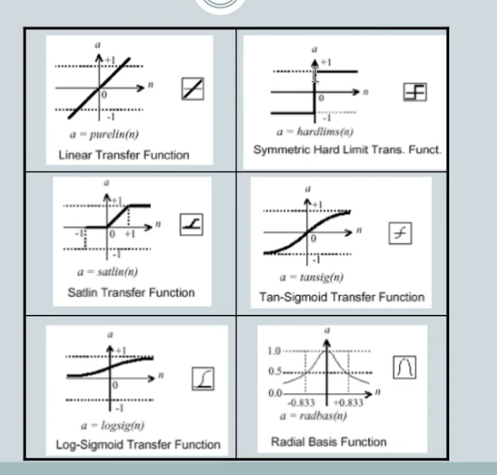
\includegraphics{4.3.png}
		\caption{Aktifleştime fonksiyonları.}
		\cite{youtube}
	\end{figure}
	
	\newpage Yukarıda gördüğünüz fonksiyonlar aktivleştime fonksiyonları içinde kullanılan fonksiyonlardır.
	
	\textbf{Tek katmanlı Yapay Sinir Ağları :}En basit ağ tipi olup bir çıktı katmanı ve buna bağlı bir girdi katmanından oluşmaktadır.Ara katman bulundurmaz.
	\begin{figure}[!h]
		\centering
		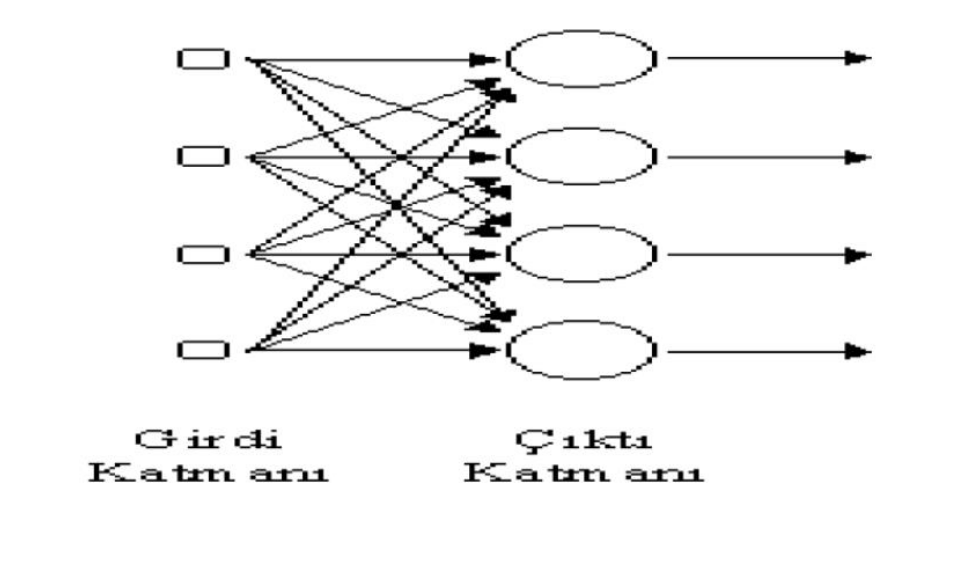
\includegraphics{4.8.png}
		\caption{Tek katmanlı Yapay Sinir Ağları.}
		\cite{SlideServe}
	\end{figure}
	\newline Bu tür ağ tipiyle basit problemleri çözebiliriz.
	Örnek olarak aşağıda a,b değişkenlerini and ve or kapısına soktuktan sonraki çıktıları inceliyoruz.
	\begin{figure}[!h]
		\centering
		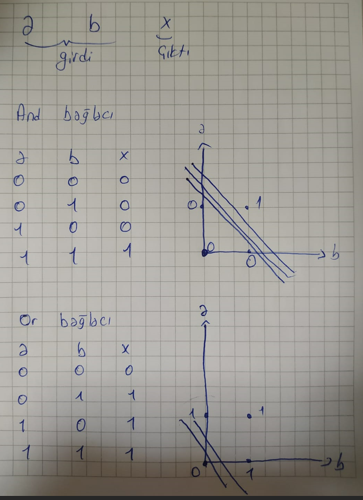
\includegraphics{4.9.png}
		\caption{Tek katmanlı Yapay Sinir Ağları çözümleri.}
	\end{figure}
	\newpage Yukarıdaki resimde de görebileceğiniz üzere a ve b değişkenlerini iki boyutlu düzleme yerleştirdiğimizde 0 ve 1 değerlerini bir soğru yardımıyla birbirinden ayırabiliyoruz.
	\begin{figure}[!h]
		\centering
		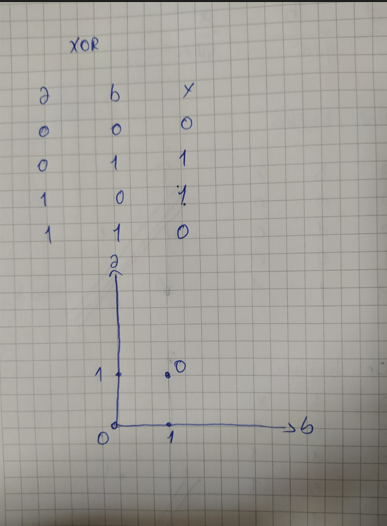
\includegraphics{4.10.png}
		\caption{Çok katmanlı Yapay Sinir Ağları çözümleri.}
	\end{figure}
	\newpage Lakin yukarıdaki problemi (XOR kapısına sokulmuş değişkenler) tek katmanlı yapay sinir ağlarıyla çözemezsiniz.Tek bir doğru ile 0 ve 1 noktalarını birbirinden ayıramazsınız.Burada devreye Çok Katmanlı Yapay Sinir Ağları giriyor.
	\newline \textbf{Çok katmanlı Yapay Sinir Ağları :}Girdi katmanı ile çıktı katmanı arasında ara katman veya katmanların olmasıdır.
	\newpage
	\begin{figure}[!h]
		\centering
		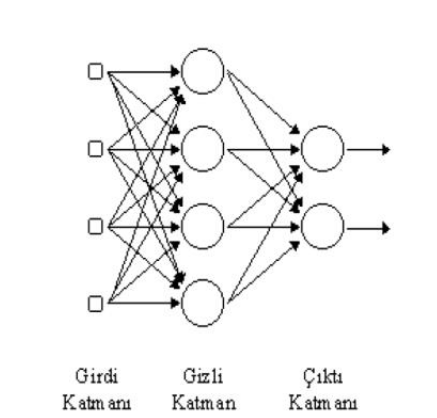
\includegraphics{4.11.png}
		\caption{Çok katmanlı Yapay Sinir Ağları.}
		\cite{SlideServe}
	\end{figure}
	\newpage Çok katmanlı Yapay Sinir Ağları daha karmaşık problemleri çözmek için tasarlanmıştır.Bundan dolayıda eğitilmesi daha zordur ve daha çok zaman alır.
	\newline \textbf{Yapay Sinir Ağlarında Bias kavramı:}Bias skaler bir değerdir.İnput fonksiyonunda değerlerimize eklenir.Doğrunun özelliğini değiştirmez sadece kaydırma işlemi yapar.
	Bu hafta geçen haftalarda Random Forest algoritmasıyla yaptığım çalışmamı Yapay Siniar ağlarına taşıdım.Yapay Sinir Ağlarına geçen hafta değindiğim için bu hafta değinmeyeceğim.
	\newline \textbf{Alınan Hatalar:} \textbf{AttributeError: module 'tensorflow.python.distribute.input lib' has no attribute 'DistributedDatasetInterface'. Did you mean: 'DistributedDatasetSpec'?
	} Projede Tensorflow 2.16.1 sürümü kullanılmakta. Lakin DistributedDatasetInterface özelliği 2.13 sürümlerinin altında çalışmakta.PyChar Tensorflow 2.13 öncesi sürümleri indirirken hata verdi. Daha sonra Google Colab da kodları çalıştırdık.
	\begin{figure}[!h]
		\centering
		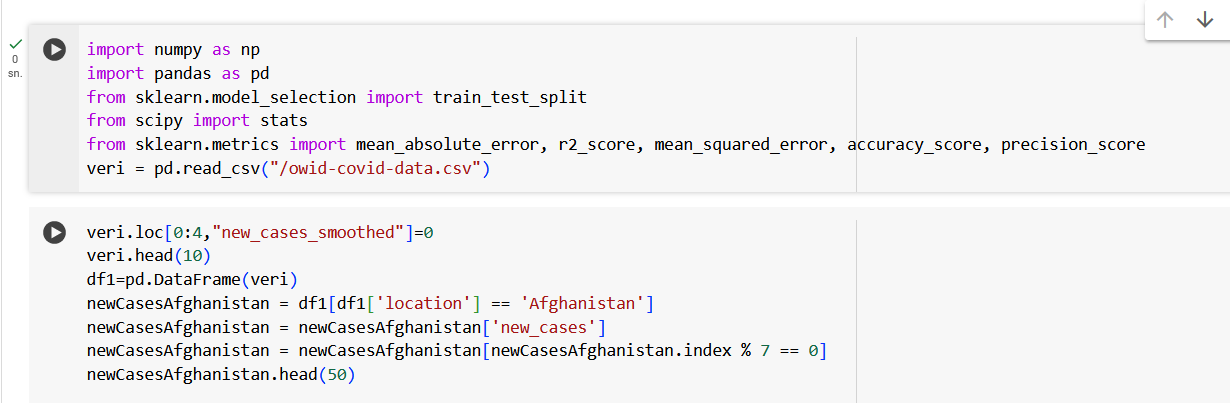
\includegraphics{5.2.png}
		\caption{Kütüphanelerin eklenmesi ve verilerin okunması.}
	\end{figure}
	\newline Yukarıdaki kodlarda kütüphanelerimi ekledik ve verilerimizi okumaya başladık.
	\begin{figure}[!h]
		\centering
		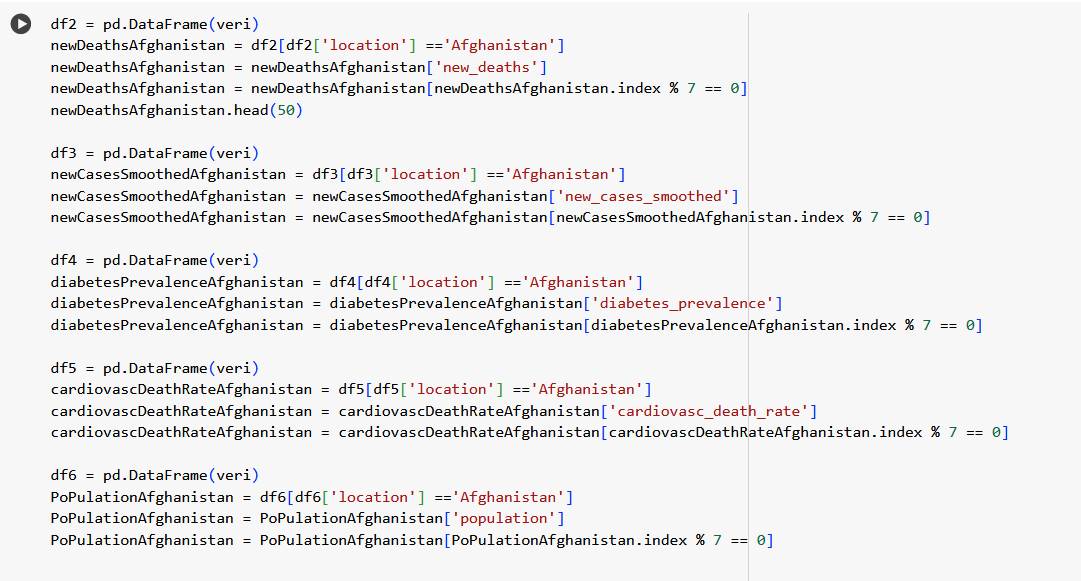
\includegraphics{5.3.png}
		\caption{Verilerin okunması.}
	\end{figure}
	\newpage Daha sonra algoritmamızda kullanacağımız diğer verilerdi de okuduk.
	
	\begin{figure}[!h]
		\centering
		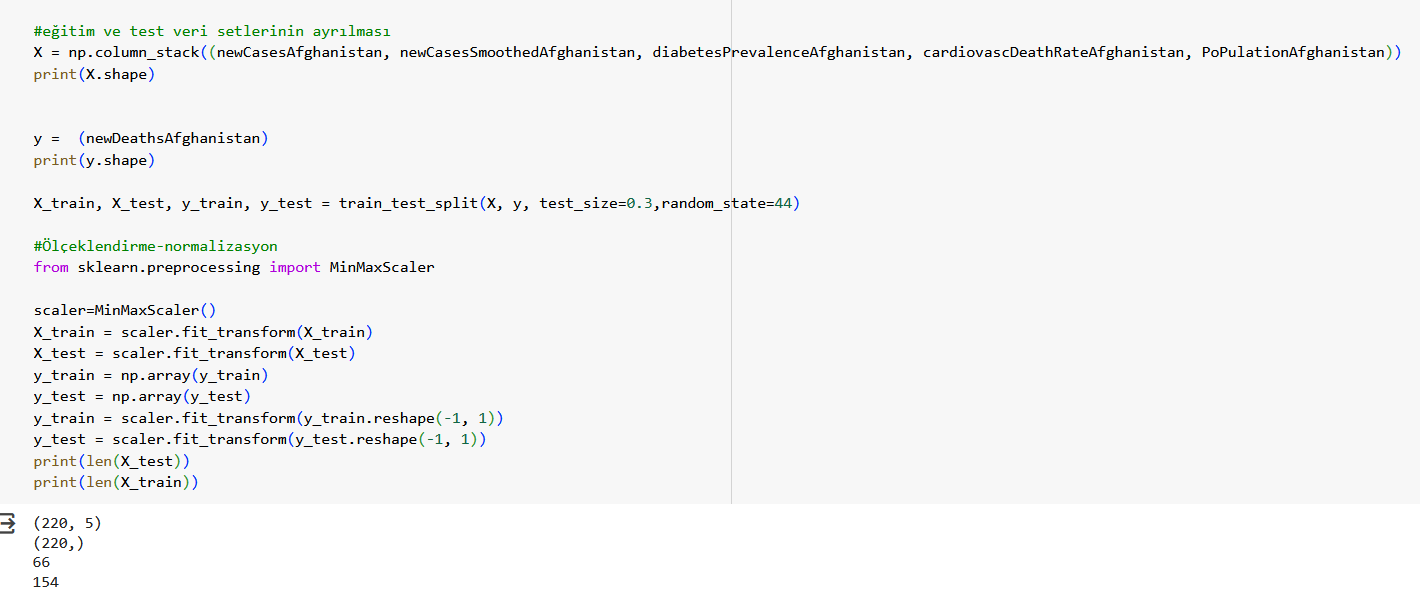
\includegraphics{5.4.png}
		\caption{Verilerin ayrıştırılması ve hazırlanması}
	\end{figure}
	\newpage
	Bağımlı ve bağımsız değişkenlerimizi hazırladıktan sonra verilerimizi \%30 u test verisi olacak şekilde ayırıyoruz. X\_train ve y\_train eğitimde kullanacağımız verilerimizi içerir.X\_test ve y\_test ise test verilerimizi içerir. Daha sonra verilerimiz üstündeki dönüşümleri yapıyoruz.
	
	\begin{figure}[!h]
		\centering
		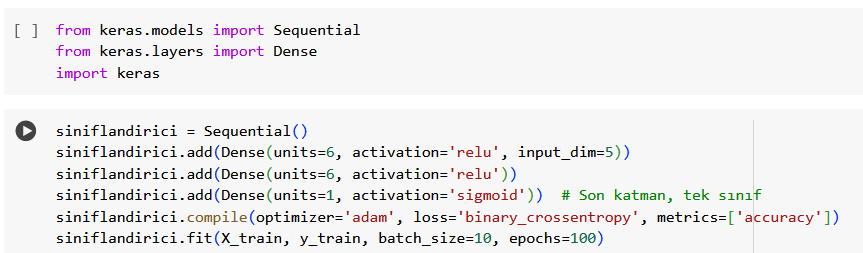
\includegraphics{5.5.png}
		\caption{Modelimizin oluşturulması}
	\end{figure}
	\newpage
	Yapay Sinir ağları modelimiz için gerekli olan kütüphaneleri çalışmamıza ekliyoruz. Daha sonra siniflandirici nesnesi oluşturuyoruz.Add komutuyla katman ekliyoruz.Units parametresi nöron sayısımı activation ise aktivasyon fonksiyonumuzu temsil ediyor.En son olarak da fit metotuyla sistemimizi eğitiyoruz.
	
	\begin{figure}[!h]
		\centering
		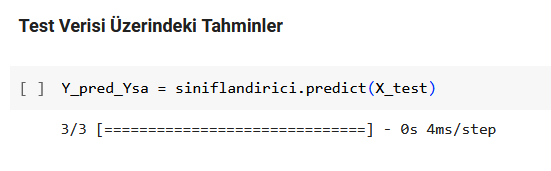
\includegraphics{5.6.png}
		\caption{Modelden tahmini değerler elde etme.}
	\end{figure}
	Eğittiğimiz modele X\_test verilerimiz besleyerek çıktıları alıyoruz.
	
	
	\begin{figure}[!h]
		\centering
		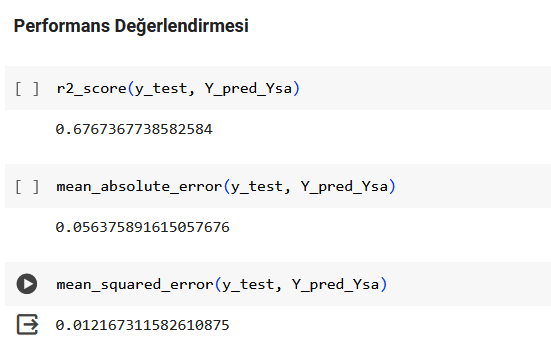
\includegraphics{5.7.png}
		\caption{Modelin performansını değerlendirme.}
	\end{figure}
	\newpage Daha sonra eğittiğimiz modelden elde ettiğimiz test sonuçları ile gerçek test verilerimizi karşılaştırarak r2, mean absolute error, mean squared error metriklerinde değerlendiriyoruz.
	
	
	\begin{figure}[!h]
		\centering
		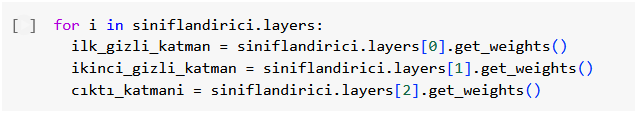
\includegraphics{5.8.png}
		\caption{Ağırlıkların bulunması.}
	\end{figure}
	\newpage
	\begin{figure}[!h]
		\centering
		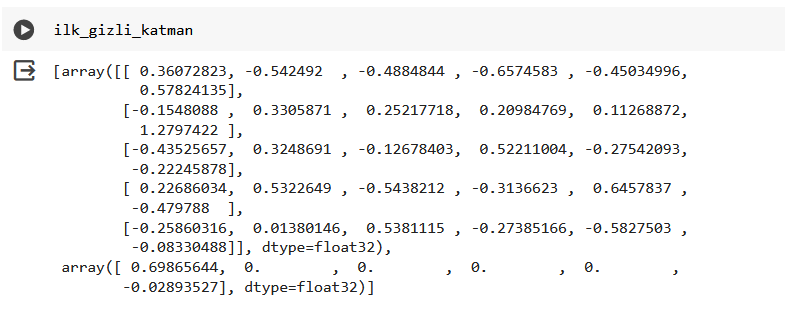
\includegraphics{5.9.png}
		\caption{Ağırlıkların bulunması.}
	\end{figure}
	
	\begin{figure}[!h]
		\centering
		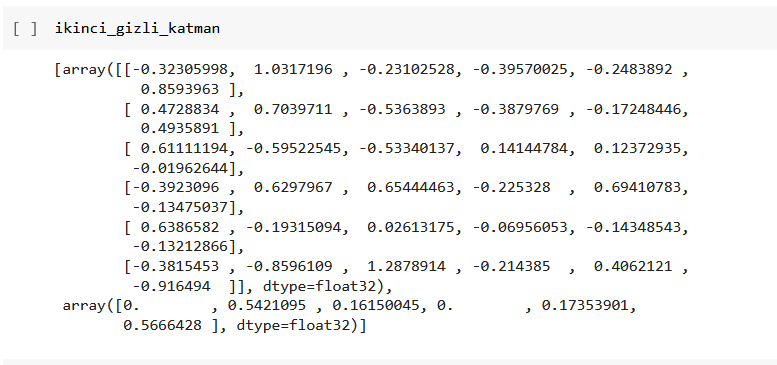
\includegraphics{5.10.png}
		\caption{Ağırlıkların bulunması.}
	\end{figure}
	\newpage
	\begin{figure}[!h]
		\centering
		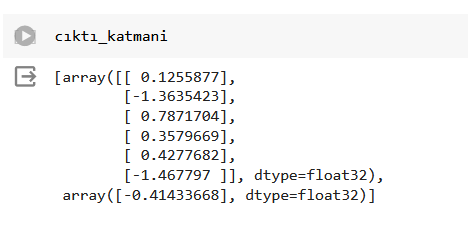
\includegraphics{5.11.png}
		\caption{Ağırlıkların bulunması.}
	\end{figure}
	Yukarıdaki kodlarda ise nöronlar arasındaki ağırlıkları buluyoruz.Her katmanın ayrı ayrı hesaplayıp çıktısını inceliyoruz.\cite{youtube-ysa}
	Geçen haftaki çalışmamızda yapay sinir ağları ile bir model oluşturup verimiz üzerinde çalıştırmıştık. Bu hafta ise yapar sinir ağları parametre ayarları hakkında araştırma yapıldı.Öncelikle aktivasyon fonksiyonlarından bahsedeceğiz.
	\newline \textbf{Aktivasyon fonksiyonları:}Yapay sinir ağlarında kullanılan aktivasyon fonksiyonları, her bir katmanın çıktılarını non-lineer hale getirerek sinir ağının daha karmaşık ilişkileri öğrenmesine olanak tanır.
	Aşağıda sık kullanılan Aktivasyon kodlarından bahsedilmiştir.
	\newline 
	\newline \textbf{1. Binary Step Fonksiyonu:}Binary Step Fonksiyonu ikili sınıflandırma durumunda kullanılır. Çoklu sınıflandırmada işe yaramaz. Genellikle çıkış katmanlarında (Output Layer) kullanılır.
	\begin{figure}[!h]
		\centering
		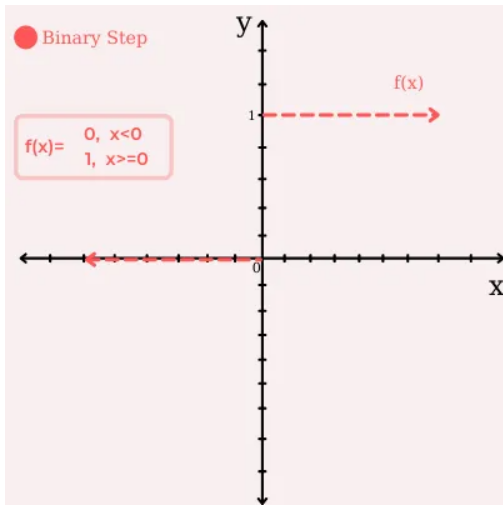
\includegraphics{6.1.png}
		\caption{Binary Step fonksiyonu.}
	\end{figure}
	\newline Türevi sıfır olduğu için de Geri Yayılım(Back Propagation) sırasında parametreler güncellenmez yani öğrenme işlemi gerçekleşmez. Bu yüzden de Gizli Katmanlarda(Hidden Layers) tercih edilmez.Fonksiyonumunuz türevi bizim için önemlidir.
	\newline \textbf{Lineer Fonksiyon:} Model optimizasyonu sırasında, türevi sabit bir değere eşit olacağı için öğrenme işlemi istenilen başarımı göstermeyecektir. Bu yüzden bu fonksiyon çok basit görevler dışında kullanılması tercih edilmez.	
	\begin{figure}[!h]
		\centering
		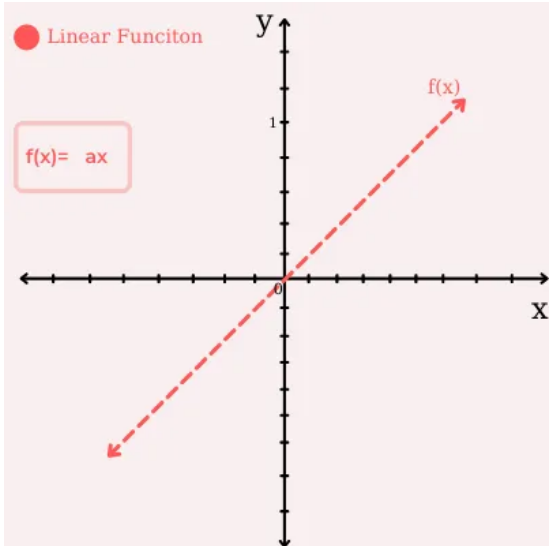
\includegraphics{6.2.png}
		\caption{Lineer fonksiyon.}
	\end{figure}
	\newline \textbf{Sigmoid Fonksiyonu:}En çok kullanılan aktivasyon fonksiyonlarından birisidir. Şimdiye kadar bahsettiğimiz ilk doğrusal olmayan(non-linear) fonksiyondur. Karar vermeye yönelik olasılıksal bir yaklaşımdır ve değer aralığı [0,1] arasındadır. Yani çıktının hangi sınıfa ait olduğuna dair olasılıksal bir değer verir bize. Sigmoid fonksiyonu sürekli yani türevlenebilir bir fonksiyon olduğundan öğrenme işlemi gerçekleşir.
	\newline $ g(x) = 1/(1+e^(-x)) $
	
	\begin{figure}[!h]
		\centering
		\includegraphics{6.3.png}
		\caption{Sigmoid fonksiyonu.}
	\end{figure}
	\newpage Fakat Sigmoid de mükemmel değildir. Çünkü türev değeri, tablodan da görebildiğimiz üzere, uç noktalarda sıfıra yakınsar (Vanishing Gradient).Bu durum Back Propagation sırasında öğrenmenin durmasına sebebiyet verir . Bu sebeple çok katmanlı ağlarda kullanılması tavsiye edilmez.
	\newline \textbf{Hiperbolik Tanjant(tanh):} Sigmoid fonksiyonu ile oldukça benzerdir. Bu fonksiyon da ikili sınıflandırma için kullanılır. Fakat tanh [-1,1] değer aralığında değerler alır ve orjin etrafında simetriktir.
	\newline $tanh(x) = 2sigmoid(2x)-1$
	\begin{figure}[!h]
		\centering
		\includegraphics{6.4.png}
		\caption{Hiperbolik Tanjant fonksiyonu.}
	\end{figure}\newpage
	Grafikten gördüğümüz üzere, uç noktalarda türev sıfıra yakınsar. Yani tanh fonksiyonu da Vanishing Gradient probleminden muzdariptir. Model kurulacağı zaman katman sayısı dikkate alınmalıdır, çok katmanlı ağlarda tercih edilmemelidir.
	\newline \textbf{ Rectified Linear Unit (RELU):}Bir diğer fonksiyonumuz Rectifier Linear Unit. Genellikle Convolutional Neural Network (CNN)’te ve ara katmanlarda çok sık kullanılan ReLU fonksiyonunun ana avantajı aynı anda tüm nöronları aktive etmemesidir. Yani bir nöron negatif değer üretirse, aktive edilmeyeceği anlamına gelir.
	\begin{figure}[!h]
		\centering
		\includegraphics{6.5.png}
		\caption{RELU fonksiyonu.}
	\end{figure}
	ReLU’nun türevi sıfıra yakınsamadığı için önceki fonksiyonlarda gördüğümüz Vanishing Gradient probleminden etkilenmez. Fakat ReLU da mükemmel değildir.
	\newpage
	Grafiğe baktığımızda, fonksiyonun türevinin negatif değerlerde sıfır olduğunu görürüz. Daha önceki fonksiyonlarda da bahsettiğimiz gibi bu durum Geri Yayılım (Back Propagation) esnasında parametrelerimizin güncellenmeyeceği, yani öğrenme işleminin olmayacağı anlamına gelir. Bu probleme Dying ReLU adı verilir. Bu problemi çözmek için relu fonksiyonlarının farklı	varyasyonları geliştirilmiştir.\cite{Aktivasyon}
	
	Geçen haftaki çalışmamızda ölçeklendirmeyi tüm bağımlı X dizisi için yapmıştık fakat bu çok büyük değerler içeren (örneğin population) parametrelerin diğer parametreleri 0 a yakınsamasına yol açacaktı.Bunun için tüm parametreleri ayrı ayrı ölçeklendirip daha sonra X bağımlı değişken dizisine koyduk.
	\begin{figure}[!h]
		\centering
		\includegraphics{6.6.png}
		\caption{Bağımlı değikenlerimizi ayrı ayrı ölçeklendirme.}
	\end{figure}
	\newpage Modelimize besleyeceğimiz değerleri bu şekilde ölçeklendirdik.Daha sonra en başarılı aktivasyon fonksiyonunu bulmak için grid search yöntemini uyguladık.
	\begin{figure}[!h]
		\centering
		\includegraphics{6.7.png}
		\caption{Grid Searh yöntemi için parametreler.}
	\end{figure}
	\begin{figure}[!h]
		\centering
		\includegraphics{6.8.png}
		\caption{Grid Searh yöntemi uygulanması.}
	\end{figure}
	\newpage
	Bu şekilde tüm katmanlarda 3 farklı aktivasyon fonksiyonu deneyerek en düşük hata oranına sahip olanı bulmaya çalıştık. Fakat bu kodun dezavantajı tüm katmanlarda aynı aktivasyon fonksiyonunu kullandık.
	Farklı aktivasyon fonksiyonları için r2 score,mean absolute error, mean squared error değerleri aşağıdaki tabloda gösterilmiştir.
	
	\begin{table}[h!]
		\centering
		\caption{Aktivasyon Fonksiyonlarının Performans Karşılaştırması}
		\label{tab:performance_comparison}
		\begin{tabular}{lllll}
			\hline
			Akt Fonksiyonları  & r2score & mae & mse & eğitim zamanı \\ \hline
			Relu & 0.732 & 0.054 & 0.010 & 7.72 saniye\\
			Sigmoid & -0.042 & 0.092 & 0.039 & 13.45 saniye \\
			Tanh & 0.573 & 0.061 & 0.016 & 11.48 saniye\\ 
			\hline
		\end{tabular}
		\caption*{Tablo notları: Bu tablo, farklı aktivasyon fonksiyonlarının performans metriklerini göstermektedir.}
	\end{table}
	\newpage
	Modelimizin başarımı için kullandığımız metrikleri (Ölçütleri) incelemek çıkan sonuçları yorumlamamızda yardımcı olacaktır.Bu yüzden kullandığımız ölçütleri inceleyeceğiz.
	
	\textbf{R²:}R², verilerin yerleştirilmiş regresyon hattına ne kadar yakın olduğunun istatistiksel bir ölçüsüdür. Ayrıca belirleme katsayısı veya çoklu regresyon için çoklu belirleme katsayısı olarak da bilinir. Daha basit bir dilde söylemek gerekirse R-kare, doğrusal regresyon modelleri için uygunluk ölçüsüdür.
	\begin{figure}[!h]
		\centering
		\includegraphics[width=0.8\textwidth, height=0.4\textheight]{6.9.png}
		\caption{R² metriği.}
	\end{figure}\cite{r2}
	\newpage
	\begin{equation}
		R^2 = 1 - \frac{SS_{res}}{SS_{tot}}
	\end{equation}
	\begin{center}
		\textbf{(1)} Burada, $SS_{res}$ tahmin hatalarının karelerinin toplamını, $SS_{tot}$ ise gerçek değerlerin ortalamadan sapmalarının karelerinin toplamını temsil eder.
	\end{center}
	\textbf{Düzeltilmiş(Adjusted) R²:}Düzeltilmiş R2, modelin karmaşıklığını (bağımsız değişkenlerin sayısını) göz önünde bulundurarak R2R2 değerini ayarlar. Bu, modeldeki gereksiz değişkenlerin etkisini azaltır ve modelin genel performansını daha doğru bir şekilde değerlendirmeyi sağlar.\cite{Duzelr2}
	
	Düzeltilmiş \( R^2 \) denklemi:
	\[
	\bar{R}^2 = 1 - \left( \frac{(1 - R^2)(n - 1)}{n - k - 1} \right)
	\]
	\begin{align*}
		n &= \text{gözlem sayısı} \\
		k &= \text{bağımsız değişken sayısı}
	\end{align*}
	
	
	
	
	
	\textbf{Ortalama Mutlak Hata (Mean Absolute Error - MAE:} Bir tahmin modelinin gerçek değerlerle ne kadar uyumlu olduğunu ölçen bir performans metriğidir. Bu metrik, tahmin edilen değerler ile gerçek değerler arasındaki farkların mutlak değerlerinin ortalamasını verir. Yani, her tahminin gerçek değerden ne kadar sapma gösterdiğini ölçer ve bu sapmaların ortalamasını alır.
	\[
	\text{MAE} = \frac{1}{n} \sum_{i=1}^{n} \left| x_i - \bar{x} \right|
	\]
	\begin{align*}
		n &= \text{gözlem sayısı} \\
		x_i &= \text{veri noktasının değeri} \\
		\bar{x} &= \text{veri noktalarının ortalaması}
	\end{align*}
	\newpage \textbf{Ortalama Karesel Hata (MSE – Mean Squared Error):}
	
	Ortalama Karesel Hata, tahmin edilen değerler ile gerçek değerler arasındaki farkların karelerinin ortalaması alınarak hesaplanır. MSE, büyük hatalara daha fazla ağırlık verir, bu nedenle modelin büyük sapmalarını sert bir şekilde cezalandırır. Bu özellik, modelinizin büyük hatalar yapmasını özellikle önlemek istediğiniz durumlarda yararlıdır.\cite{MSE}
	\[
	\text{MSE} = \frac{1}{n} \sum_{i=1}^{n} (y_i - \hat{y}_i)^2
	\]
	\begin{align*}
		n &= \text{gözlem sayısı} \\
		y_i &= \text{gerçek değer} \\
		\hat{y}_i &= \text{tahmin edilen değer}
	\end{align*}
	Projenin en sonunda SVR(Support Vector Regression) algoritması da çalışmalara eklenmiştir. Algoritmanın çıktılarını ve nasıl çalıştığını daha iyi anlamak için SVR makine öğrenmesi algoritması kısaca anlatılacaktır.
	\textbf{SVR(Support Vector Regression):}Destek vektör algoritması ilk başta sınıflandırma için çıkmış bir algoritma olmasına rağmen regresyon için de kullanılmaktadır. Sınıflandırma işlemleri için SVM yani Support Vector Machine kullanılırken regresyon için de Support Vector Regression kullanılmaktadır.
	\begin{figure}[!h]
		\centering
		\includegraphics[width=0.8\textwidth, height=0.3\textheight]{6.13.png}
		\caption{Sigmoid fonksiyonu.}
	\end{figure}
	\newpage
	Amaç, bir marjın aralığına maksimum noktayı en küçük hata ile alabilecek şekilde doğru ya da eğriyi belirlemektir. Yani, Destek vektör regresyonu uyguladığımızda, çizeceğimiz aralığın maksimum noktayı içerisine almasını sağlamaktır. Burada doğrusal ve doğrusal olmayan olarak iki türlü SVR metodu bulunmaktadır.\cite{svr}
	\newline
	En son olarakta veri setimizdeki Afganistan verilerini ve tüm verileri(218 farklı ülke için toplam 55322 veri) kullanarak Random Forest , Neural Network ve Support Vector Regression algoritmaları ile modeller oluşturulmuştur.
	Algoritmalarla tüm veriler için model oluştururken eksik veri sorunu ile karşılaşıldı fakat bu sorun eksik verilerin bağlı oldukları sütun ortalamaları ile doldurulmasıyla kısmen çözüldü.
	
	\begin{table}[h!]
		\centering
		\caption{MSE Karşılaştırması}
		\label{tab:performance_comparison}
		\begin{tabular}{llll}
			\hline
			& Random Forest & NN & SVR\\ \hline
			Afganistan & 1008.05 & 0.01458 &0.01458 \\
			Tüm veriler & 190374 & 0.00056 & 0.00330  \\ 
			\hline
		\end{tabular}
		\caption*{Tablo notları: Bu tabloda, Afganistan ve tüm veriler için 3 farklı algoritmanın Mean squared error metriği karşılaştırılmıştır.}
	\end{table}
	
	\begin{table}[h!]
		\centering
		\caption{MAE Karşılaştırması}
		\label{tab:performance_comparison}
		\begin{tabular}{llll}
			\hline
			& Random Forest & NN & SVR\\ \hline
			Afganistan & 18.7669.05 & 0.05067 &0.08372 \\
			Tüm veriler & 27.8525 & 0.00168 & 0.05029  \\ 
			\hline
		\end{tabular}
		\caption*{Tablo notları: Bu tabloda, Afganistan ve tüm veriler için 3 farklı algoritmanın Mean absolute error metriği karşılaştırılmıştır.}
	\end{table}
	
	\begin{table}[h!]
		\centering
		\caption{Eğitim süresi karşılaştırılması}
		\label{tab:performance_comparison}
		\begin{tabular}{llll}
			\hline
			& Random Forest & NN & SVR\\ \hline
			Afganistan & 0.21 saniye & 8.93 saniye & 0.01 saniye \\
			Tüm veriler & 12.69 saniye &863.59 saniye & 1.82 saniye  \\ 
			\hline
		\end{tabular}
		\caption*{Tablo notları: Bu tabloda, Afganistan ve tüm veriler için 3 farklı algoritmanın eğitim süreleri karşılaştırılmıştır.}
	\end{table}
	\section{Sonuç:}Sonuç olarak bu çalışmada 2 farklı veri kümesi ve 3 farklı yapay zeka algoritması kullanarak hastalık durumundaki vefat sayısı tahmin etmeye çalıştık.Yukarıdaki Tablo 2 Tablo 3 ve Tablo 4 de de görebileceğiniz üzere bizim veri setimizde en başarılı algoritma Yapay Sinir Ağları seçildi. 
	\section{Teşekkürler:}Çalışmamın her aşamasında desteklerini hiçbir zaman esirgemeyen değerli hocam Emre GÜNGÖR'e teşekkürler.
	\newpage
	
	\bibliographystyle{ieeetr}
	\bibliography{document_vize.bib}
	
	
	
	
	
\end{document}
